\documentclass[11pt,a4paper]{article}

% ----------------------------------------------------------------------
% Codificación e idioma
% ----------------------------------------------------------------------
\usepackage[utf8]{inputenc}
\usepackage[T1]{fontenc}
\usepackage[main=spanish,provide=*]{babel}
\usepackage[expansion=false]{microtype}

% ----------------------------------------------------------------------
% Matemática
% ----------------------------------------------------------------------
\usepackage{amsmath,amssymb,amsthm}
\usepackage{mathtools}

% ----------------------------------------------------------------------
% Gráficos: TikZ y pgfplots
% ----------------------------------------------------------------------
\usepackage{tikz}
\usepackage{tikz-3dplot}
\usepackage{pgfplots}
\pgfplotsset{compat=1.18}
\usetikzlibrary{calc,arrows.meta,positioning,decorations.markings,
                3d,backgrounds,fadings,shapes.geometric,patterns}

% ----------------------------------------------------------------------
% Página, color, enlaces
% ----------------------------------------------------------------------
\usepackage[margin=2.4cm]{geometry}
\usepackage{xcolor}
\usepackage{graphicx}
\usepackage{caption}
\usepackage{enumitem}
\usepackage{booktabs}
\usepackage{tabularx}
\usepackage{placeins}
\usepackage{float}
\usepackage{fancyhdr}
\usepackage[most]{tcolorbox}
\usepackage{hyperref}

% ----------------------------------------------------------------------
% Paleta
% ----------------------------------------------------------------------
\definecolor{navy}{HTML}{1B2A4A}
\definecolor{azul}{HTML}{2563A8}
\definecolor{rojo}{HTML}{C0392B}
\definecolor{verde}{HTML}{1F8A4C}
\definecolor{oro}{HTML}{B8860B}
\definecolor{gris}{HTML}{7A8699}
\definecolor{hielo}{HTML}{EEF3FA}

\hypersetup{
  colorlinks=true, linkcolor=navy, urlcolor=azul, citecolor=azul,
  pdftitle={Coordenadas homogéneas y dualidad en geometría proyectiva},
  pdfauthor={Carlos Nexans}
}

\captionsetup{font=small,labelfont={bf,color=navy},textfont=it}

% Títulos de sección en color
\usepackage{titlesec}
\titleformat{\section}{\normalfont\Large\bfseries\color{navy}}{\thesection.}{0.6em}{}
\titleformat{\subsection}{\normalfont\large\bfseries\color{azul}}{\thesubsection}{0.6em}{}
\titlespacing*{\section}{0pt}{1.4ex plus 1ex minus .2ex}{1ex}

% Encabezado / pie
\pagestyle{fancy}
\fancyhf{}
\renewcommand{\headrulewidth}{0pt}
\fancyfoot[C]{\small\color{gris}\thepage}

% ----------------------------------------------------------------------
% Entornos para teoremas / definiciones
% ----------------------------------------------------------------------
\newtcolorbox{teorema}[1][]{
  enhanced, colback=navy, colframe=oro, boxrule=1pt, arc=2pt,
  left=10pt,right=10pt,top=8pt,bottom=8pt,
  fontupper=\color{white}, #1}

\newtcolorbox{defbox}[1][]{
  enhanced, colback=hielo, colframe=azul, boxrule=1pt, arc=2pt,
  left=10pt,right=10pt,top=7pt,bottom=7pt, #1}

\newtcolorbox{codebox}[1][]{
  enhanced, colback=navy!4, colframe=gris!55, boxrule=0.8pt, arc=1pt,
  left=10pt,right=10pt,top=6pt,bottom=6pt,
  fontupper=\ttfamily\small, #1}

% Notación
\newcommand{\RP}{\mathbb{RP}}
\newcommand{\R}{\mathbb{R}}
\newcommand{\inc}[2]{\langle #1,\, #2\rangle}
\newcommand{\hp}[3]{[#1\,{:}\,#2\,{:}\,#3]}
\newcommand{\hpf}[4]{[#1\,{:}\,#2\,{:}\,#3\,{:}\,#4]}

% ======================================================================
\begin{document}

% ----------------------------------------------------------------------
% Portada
% ----------------------------------------------------------------------
\begin{titlepage}
\thispagestyle{empty}
\begin{tikzpicture}[remember picture,overlay]
  \fill[navy] (current page.north west) rectangle ([yshift=-5.2cm]current page.north east);
  \fill[azul!85!navy] ([yshift=-5.2cm]current page.north west)
        rectangle ([yshift=-5.55cm]current page.north east);
  \node[anchor=north west, text=white, align=left]
        at ([xshift=2.4cm,yshift=-1.6cm]current page.north west)
        {\fontsize{11}{13}\selectfont \textbf{GEOMETRÍA I\ \ {\color{azul!40!white}$\cdot$}\ \ LICENCIATURA EN MATEMÁTICA}};
  \node[anchor=north west, text=white, align=left]
        at ([xshift=2.35cm,yshift=-2.3cm]current page.north west)
        {\fontsize{30}{34}\selectfont\bfseries Coordenadas homogéneas};
  \node[anchor=north west, text=white, align=left]
        at ([xshift=2.35cm,yshift=-3.3cm]current page.north west)
        {\fontsize{30}{34}\selectfont\bfseries y dualidad};
  \node[anchor=north west, text=oro!85!white, align=left]
        at ([xshift=2.4cm,yshift=-4.4cm]current page.north west)
        {\fontsize{15}{18}\selectfont\itshape en la geometría proyectiva del plano};
\end{tikzpicture}

\vspace{8.5cm}

\noindent

\begin{tikzpicture}
  \node[anchor=west, text=navy, align=left] at (0,0)
    {\large\bfseries Trabajo de investigación};
\end{tikzpicture}

\vspace{0.4cm}
\noindent\large
Autor: \textbf{Carlos Nexans}\\[2pt]
Materia: \textbf{Geometría I} — Licenciatura en Matemática\\[2pt]
Institución: \textbf{UCAECE}\\[2pt]
Tema: coordenadas homogéneas (\textnumero\,7) y dualidad (\textnumero\,4)\\[2pt]
Fecha de exposición: \textbf{martes 9 de junio de 2026}

\vfill
\noindent\color{gris}\small
Documento generado en \LaTeX{} con figuras vectoriales en Ti\emph{k}Z.
\end{titlepage}

% ----------------------------------------------------------------------
% Índice
% ----------------------------------------------------------------------
\tableofcontents
\thispagestyle{fancy}
\vspace{1cm}

\noindent\color{gris}\small
\textit{Resumen.} Este trabajo combina dos temas de la geometría proyectiva
del plano que están íntimamente ligados: las \textbf{coordenadas
homogéneas}, que dan un lenguaje algebraico para puntos, rectas y el
infinito, y el \textbf{principio de dualidad}, que la simetría de esas
coordenadas convierte en un teorema demostrable. Tras la fundamentación
teórica se presentan ejemplos trabajados, las homografías como
transformaciones que preservan la incidencia y aplicaciones modernas:
desde el modelo de cámara estenopeica $\lambda\,[u,v,1]^\top=K[R\mid t]\,[X,Y,Z,1]^\top$
hasta un visor propio de nubes de puntos LiDAR para conducción autónoma.
\color{black}

\clearpage

% ======================================================================
\section{Introducción}
% ======================================================================

La \textbf{geometría proyectiva} estudia las propiedades de las figuras que
se conservan bajo proyección: aquello que un pintor o una cámara preservan
al proyectar el mundo tridimensional sobre un lienzo o un sensor plano. A
diferencia de la geometría euclidiana, no se ocupa de distancias ni de
ángulos, sino de relaciones de \emph{incidencia} —qué puntos están sobre
qué rectas— y de \emph{colinealidad} y \emph{concurrencia}.

La diferencia más llamativa con la geometría euclidiana es el tratamiento
del paralelismo. En el plano usual, dos rectas paralelas no se cortan; la
intersección de dos rectas es una regla con una excepción. La geometría
proyectiva elimina esa excepción agregando, para cada dirección, un
\textbf{punto al infinito} donde se cortan todas las rectas paralelas a
ella. En el plano proyectivo
\[
  \text{dos rectas distintas siempre se cortan en exactamente un punto.}
\]
Esta uniformidad tiene una consecuencia profunda: punto y recta pasan a
desempeñar papeles \emph{simétricos}, y esa simetría es el corazón de este
trabajo.

\subsection{Contexto histórico}
\label{sec:historia}

Las raíces de la disciplina están en el estudio de la perspectiva durante
el Renacimiento, cuando pintores como Brunelleschi, Alberti y, sobre todo,
Piero della Francesca enfrentaron de manera sistemática el problema de
dibujar el espacio sobre una superficie plana. Su práctica fue convertida en
matemática en cuatro saltos que conviene tener presentes.

\begin{description}[leftmargin=0pt,style=nextline]
\item[1639 — Girard Desargues (1591--1661).]
  Sienta las bases de la geometría proyectiva al estudiar la perspectiva
  con herramientas matemáticas. Introduce de modo natural los puntos al
  infinito y demuestra el teorema que hoy lleva su nombre sobre triángulos
  homológicos (Sección~\ref{sec:desargues}). Su obra pasa desapercibida
  durante casi dos siglos.
\item[1822 — Jean-Victor Poncelet (1788--1867).]
  Recupera y sistematiza la disciplina en su \emph{Traité des propriétés
  projectives des figures}. Enuncia y aplica el \textbf{principio de
  dualidad} como herramienta de descubrimiento.
\item[1872 — Felix Klein (1849--1925).]
  En el \emph{Programa de Erlangen} entiende cada geometría como el estudio
  de los invariantes de un grupo de transformaciones. La geometría
  proyectiva queda situada como la más básica de una jerarquía: fijando una
  recta del infinito se obtiene la afín; fijando además una forma cuadrática
  sobre ella, la euclidiana.
\item[Siglos XX y XXI — visión por computadora y gráficos.]
  La proyectiva se vuelve la herramienta operativa: el libro de
  \emph{Hartley \& Zisserman} (2004) la convierte en el lenguaje estándar
  de la visión por computadora; los \emph{pipelines} de GPU representan los
  vértices en coordenadas homogéneas $4\times4$; los autos autónomos fusionan
  LiDAR y cámaras mediante las mismas matrices $K[R\mid t]$ que aparecerán
  en la Sección~\ref{sec:camera}.
\end{description}

% ======================================================================
\section{Coordenadas homogéneas}
% ======================================================================

\subsection{El modelo: rectas por el origen}

La forma más limpia de construir el plano proyectivo real $\RP^2$ es a
partir de $\R^3$. Consideramos $\R^3 \setminus \{\mathbf 0\}$ y declaramos
equivalentes a dos vectores cuando son múltiplos no nulos uno del otro.
Geométricamente:

\begin{quote}
  \itshape un punto de $\RP^2$ es una recta que pasa por el origen $O$ de $\R^3$.
\end{quote}

El plano $z=1$ corta a casi todas esas rectas en un punto, y recupera así
el plano afín usual. Las rectas que viven en el plano $z=0$ no cortan a
$z=1$: representan los \textbf{puntos al infinito}, uno por cada dirección
(Figura~\ref{fig:modelo}).

\begin{figure}[ht]
\centering
\tdplotsetmaincoords{70}{115}
\begin{tikzpicture}[tdplot_main_coords,scale=2.0,
    line cap=round,line join=round,>=Latex]
  % --- plano z=0 (al fondo) ---
  \fill[gris!35,opacity=0.55] (-1.4,-1.4,0) -- (1.4,-1.4,0) --
        (1.4,1.4,0) -- (-1.4,1.4,0) -- cycle;
  \node[gris] at (1.15,1.55,0) {\small $z=0$};
  % --- ejes ---
  \draw[->,gris!80!black] (0,0,0) -- (1.85,0,0) node[anchor=north east]{\small $x$};
  \draw[->,gris!80!black] (0,0,0) -- (0,1.85,0) node[anchor=west]{\small $y$};
  \draw[->,gris!80!black] (0,0,0) -- (0,0,1.75) node[anchor=south]{\small $z$};
  % --- recta dentro de z=0 -> punto al infinito ---
  \draw[oro,very thick] (-1.3,-0.78,0) -- (1.3,0.78,0);
  \node[oro,anchor=north] at (1.2,0.74,0) {\small $\hp{x}{y}{0}$};
  % --- plano z=1 (semitransparente, encima) ---
  \begin{scope}[opacity=0.85]
  \fill[azul!25] (-1.4,-1.4,1) -- (1.4,-1.4,1) --
        (1.4,1.4,1) -- (-1.4,1.4,1) -- cycle;
  \end{scope}
  \draw[azul!55,thin] (-1.4,-1.4,1) -- (1.4,-1.4,1) --
        (1.4,1.4,1) -- (-1.4,1.4,1) -- cycle;
  \node[azul] at (1.15,1.55,1) {\small $z=1$};
  % --- rectas por el origen que cortan z=1 -> puntos ordinarios ---
  \draw[rojo,thick] (-0.55,-0.35,-1) -- (0.66,0.42,1.2);
  \fill[rojo] (0.55,0.35,1) circle (1.4pt);
  \node[rojo,anchor=south east] at (0.5,0.32,1.08) {\small $P=\hp{x}{y}{z}$};
  \draw[verde,thick] (0.45,-0.7,-1) -- (-0.54,0.84,1.2);
  \fill[verde] (-0.45,0.7,1) circle (1.4pt);
  % --- origen ---
  \fill[navy] (0,0,0) circle (1.4pt);
  \node[navy,anchor=north west] at (0.04,0,-0.04) {\small $O$};
\end{tikzpicture}
\caption{Cada punto de $\RP^2$ es una recta por el origen de $\R^3$. Las
que cortan $z=1$ son puntos ordinarios; las contenidas en $z=0$ son puntos
al infinito.}
\label{fig:modelo}
\end{figure}

\subsection{Definición de punto}

\begin{defbox}
Un punto de $\RP^2$ se escribe con \textbf{coordenadas homogéneas}
\[
  P = \hp{x}{y}{z}, \qquad (x,y,z)\neq(0,0,0),
\]
con la convención de que las ternas proporcionales representan el mismo
punto:
\[
  (x,y,z)\ \sim\ (\lambda x,\lambda y,\lambda z)
  \quad\text{para todo } \lambda\neq 0.
\]
\end{defbox}

\noindent Se usan tres números para describir un objeto con dos grados de
libertad: la escala global es irrelevante. De ahí el nombre
\emph{homogéneas}; cualquier polinomio homogéneo de grado~$d$ satisface
$f(\lambda x,\lambda y,\lambda z)=\lambda^d f(x,y,z)$, de modo que su
anulación es una propiedad bien definida sobre clases de equivalencia.

\subsection{Carta afín y puntos al infinito}
\label{sec:carta}

Si $z\neq0$ podemos normalizar dividiendo por $z$ y leer las coordenadas
cartesianas usuales:
\[
  \hp{x}{y}{z}\ \longleftrightarrow\ \left(\frac{x}{z},\,\frac{y}{z}\right)
  \qquad (z\neq 0).
\]
Cuando $z=0$ no hay punto afín asociado: $\hp{x}{y}{0}$ es el \textbf{punto
al infinito} en la dirección de pendiente $y/x$. Todas las rectas paralelas
a esa dirección comparten ese punto, y el conjunto de todos ellos forma la
\emph{recta del infinito} $\ell_\infty$. Como descomposición conjuntista,
\[
  \RP^2 \;=\; \underbrace{\R^2}_{\text{plano afín }z\neq0}
              \;\sqcup\;
              \underbrace{\ell_\infty}_{\text{direcciones, }z=0}.
\]

\begin{figure}[ht]
\centering
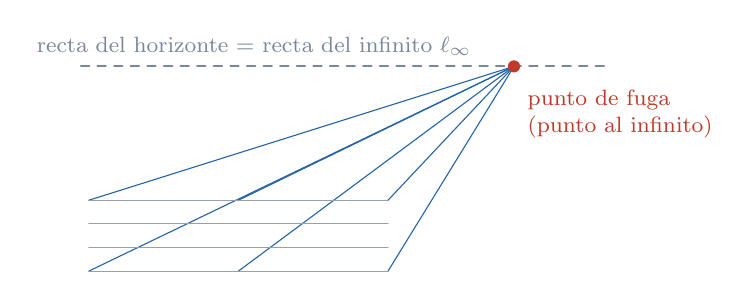
\begin{tikzpicture}[scale=1.0,>=Latex,line cap=round]
  \coordinate (V) at (5,1.6);
  % horizonte
  \draw[gris,dashed,thick] (-0.5,1.6) -- (6.2,1.6);
  \node[gris,font=\footnotesize,above] at (1.7,1.62)
        {recta del horizonte $=$ recta del infinito $\ell_\infty$};
  % rayos hacia el punto de fuga
  \foreach \x in {-0.4,1.5,3.4}{
    \draw[azul] (\x,-0.1) -- (V);
    \draw[azul] (\x,-1.0) -- (V);
  }
  % travesaños
  \foreach \y in {-0.1,-0.4,-0.7,-1.0}{
    \draw[navy!45,thin] (-0.4,\y) -- (3.4,\y);
  }
  \fill[rojo] (V) circle (2.2pt);
  \node[rojo,below right,align=left,font=\footnotesize] at ($(V)+(0.05,-0.18)$)
        {punto de fuga\\(punto al infinito)};
\end{tikzpicture}
\caption{Realización visual de la carta afín: las rectas paralelas del
suelo concurren en un \emph{punto de fuga}, que es un punto al infinito; la
recta del horizonte es la recta del infinito $\ell_\infty$.}
\label{fig:persp}
\end{figure}

\subsection{Rectas e incidencia}

Por la dualidad que estudiaremos, una recta se describe igual que un punto:
con una terna $\ell=\hp{a}{b}{c}$ salvo escala. La condición de que un
punto $P=\hp{x}{y}{z}$ esté sobre la recta $\ell=\hp{a}{b}{c}$ es

\begin{teorema}
\centering\large
$\displaystyle P\in\ell \iff \inc{P}{\ell}=ax+by+cz=0.$
\end{teorema}

\noindent La expresión $\inc{P}{\ell}=ax+by+cz$ es el producto escalar de
las dos ternas, y es \textbf{perfectamente simétrica}: intercambiar los
papeles de $P$ y $\ell$ no la altera. Esta simetría —puramente algebraica—
es la semilla de todo el principio de dualidad.

\subsection{Unir y cortar: el producto vectorial}

La estructura permite resolver dos problemas básicos con una única
operación, el producto vectorial de $\R^3$:
\[
  \underbrace{\ell = P_1\times P_2}_{\text{recta que une dos puntos}}
  \qquad\qquad
  \underbrace{P = \ell_1\times \ell_2}_{\text{punto donde se cortan dos rectas}}.
\]
En efecto, $P_1\times P_2$ es ortogonal a $P_1$ y a $P_2$, de modo que
$\inc{P_1}{\ell}=\inc{P_2}{\ell}=0$: ambos puntos están sobre $\ell$. El
caso de $\ell_1\times\ell_2$ es idéntico intercambiando los papeles
(Figura~\ref{fig:join}). Nótese que dos rectas \emph{distintas} de $\RP^2$
siempre se cortan, incluso cuando son paralelas en el sentido afín: el
producto vectorial entrega entonces un punto al infinito.

\begin{figure}[ht]
\centering
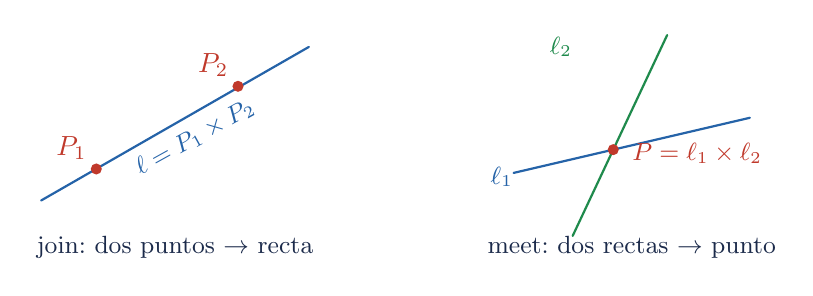
\begin{tikzpicture}[scale=1.0,>=Latex,line cap=round]
  % --- panel izquierdo: join ---
  \begin{scope}
    \draw[azul,thick] (-0.4,-0.1) -- (3.0,1.85);
    \fill[rojo] (0.3,0.3) circle (2pt) node[above left,rojo]{$P_1$};
    \fill[rojo] (2.1,1.35) circle (2pt) node[above left,rojo]{$P_2$};
    \node[azul,rotate=29] at (1.55,0.7) {\small $\ell=P_1\times P_2$};
    \node[navy] at (1.3,-0.7) {\small join: dos puntos $\to$ recta};
  \end{scope}
  % --- panel derecho: meet ---
  \begin{scope}[xshift=6.0cm]
    \coordinate (L1a) at (-0.4,0.25);
    \coordinate (L1b) at (2.6,0.95);
    \coordinate (L2a) at (0.35,-0.55);
    \coordinate (L2b) at (1.55,2.0);
    \draw[azul,thick]  (L1a) -- (L1b);
    \draw[verde,thick] (L2a) -- (L2b);
    \coordinate (P) at (intersection of L1a--L1b and L2a--L2b);
    \fill[rojo] (P) circle (2pt);
    \node[rojo,right] at ($(P)+(0.12,-0.05)$) {\small $P=\ell_1\times\ell_2$};
    \node[azul]  at (-0.55,0.2) {\small $\ell_1$};
    \node[verde] at (0.2,1.85)  {\small $\ell_2$};
    \node[navy]  at (1.1,-0.7)  {\small meet: dos rectas $\to$ punto};
  \end{scope}
\end{tikzpicture}
\caption{El mismo producto vectorial une dos puntos en una recta (izquierda)
y corta dos rectas en un punto (derecha).}
\label{fig:join}
\end{figure}

\subsection{Dimensión, subespacios y propiedades de \texorpdfstring{$\RP^n$}{RPn}}

Antes de enunciar la propiedad emblemática del plano proyectivo conviene
precisar tres ideas que usaremos repetidamente: qué quiere decir la
\emph{dimensión} de $\RP^n$, qué es un \emph{subespacio} y por qué
$\RP^n$ \emph{no} es un espacio vectorial.

\paragraph{$\RP^n$ no es un espacio vectorial.}
La construcción $\RP^n=(\R^{n+1}\setminus\{\mathbf 0\})/{\sim}$ excluye
expresamente el cero antes de cocientar, así que en $\RP^n$ no hay un
elemento neutro que jugaría el papel del vector nulo. Esa observación es
cierta, pero la razón profunda es más estructural: \emph{las operaciones
vectoriales no descienden al cociente}.
\begin{itemize}[leftmargin=1.4em,itemsep=1pt]
\item La suma $[v]+[w]$ no está bien definida sobre clases: si
  cambiamos el representante $v\leadsto\lambda v$, el resultado cambia
  (basta probar con $v=(1,0,0)$, $w=(0,1,0)$ y $\lambda=2$: se obtienen
  $\hp{1}{1}{0}$ y $\hp{2}{1}{0}$, que son puntos distintos).
\item La multiplicación escalar tampoco tiene sentido: $\lambda\cdot[v]=
  [\lambda v]=[v]$ es trivial para todo $\lambda\neq0$, y $0\cdot[v]=[0]$
  caería fuera de $\RP^n$.
\end{itemize}
Pasar al cociente proyectivo es perder la estructura lineal y quedarse
solo con relaciones de \emph{incidencia} (qué puntos están sobre qué
rectas, qué rectas pasan por qué puntos).

\paragraph{Dimensión de $\RP^n$.}
La definición es directa: si el espacio vectorial ambiente $E$ tiene
dimensión $n+1$, su \emph{proyectivización} $\mathbb P(E)$ tiene por
definición dimensión $n$. Al cocientar por la escala se pierde un grado
de libertad. Así, $\RP^2$ tiene dimensión $2$ y proviene de $\R^3$
(dimensión $3$), y $\RP^n$ proviene de $\R^{n+1}$. Equivalentemente: hacen
falta $n+1$ coordenadas homogéneas para describir un punto con $n$ grados
de libertad genuinos.

\paragraph{Subespacios proyectivos.}
La noción análoga al subespacio vectorial se obtiene proyectivizando un
subespacio del ambiente.

\begin{defbox}
Un \textbf{subespacio proyectivo} $L\subset\RP^n$ es la proyectivización
$\mathbb P(V)$ de un subespacio vectorial $V\subset\R^{n+1}$: los puntos
de $L$ son las clases de los vectores no nulos de $V$. Si $\dim V=k+1$,
entonces $\dim L = k$.
\end{defbox}
\noindent La regla cuantitativa es siempre la misma: la proyectivización
\emph{baja en uno} la dimensión, $\dim\mathbb P(V)=\dim V-1$, porque la
relación de equivalencia $v\sim\lambda v$ elimina un grado de libertad
(la escala). En $\RP^2$ la traducción es muy concreta:
\begin{itemize}[leftmargin=1.4em,itemsep=1pt]
\item un \textbf{punto} tiene dimensión $0$ y proviene de una recta por
  el origen de $\R^3$ (dimensión $1$): $1-1=0$. La intuición geométrica
  encaja con la algebraica —no podemos ``movernos'' dentro de un punto, no
  hay ninguna dirección que recorrer—;
\item una \textbf{recta} tiene dimensión $1$ y proviene de un plano por
  el origen de $\R^3$ (dimensión $2$): $2-1=1$;
\item el propio $\RP^2$ tiene dimensión $2$ y proviene de $\R^3$ completo
  (dimensión $3$): $3-1=2$.
\end{itemize}
La intersección de dos planos por el origen de $\R^3$ es una recta por el
origen: en $\RP^2$ eso se traduce, ya sin excepciones, en que dos rectas
distintas se cortan en exactamente un punto.

\paragraph{Convención $\dim\varnothing=-1$.}
El subespacio vectorial trivial $\{\mathbf 0\}\subset\R^{n+1}$ tiene
dimensión $0$, y al proyectivizarlo no queda ningún vector no nulo: su
proyectivización es el \emph{conjunto vacío}. Aplicando la regla
$\dim\mathbb P(V)=\dim V-1$ obtenemos
\[
  \dim\varnothing \;=\; \dim\mathbb P(\{\mathbf 0\})
  \;=\; 0-1 \;=\; -1.
\]
La convención no es un artificio: es lo que hace falta para que la
fórmula de dimensión que enunciaremos a continuación siga valiendo
\emph{también} cuando dos subespacios no se cortan.

\paragraph{Fórmula de dimensión y consecuencia.}
Estas tres ideas se articulan en la \emph{fórmula de dimensión} de
Santaló (§9.2). Si $L_r,M_p\subset\RP^n$ son subespacios de dimensiones
$r$ y $p$, entonces
\[
  \dim L_r + \dim M_p \;=\; \dim(L_r+M_p)+\dim(L_r\cap M_p),
\]
con la convención $\dim\varnothing=-1$. En consecuencia, si $r+p\ge n$
los dos subespacios siempre se cortan. Particularizando a $r=p=1$,
$n=2$ se obtiene la propiedad emblemática:
\begin{teorema}
\centering\large
En $\RP^2$, dos rectas distintas siempre tienen exactamente un punto común.
\end{teorema}
Otras propiedades inmediatas: por dos puntos pasa exactamente una recta;
toda recta tiene al menos tres puntos; no todos los puntos están sobre la
misma recta; por todo punto pasan al menos tres rectas. La simetría de
estos enunciados anticipa la dualidad.

% ======================================================================
\section{Dualidad}
% ======================================================================

\subsection{El principio de dualidad}

La simetría observada se cristaliza en uno de los resultados más elegantes
de toda la matemática:

\begin{teorema}
\textbf{Principio de dualidad.} Todo enunciado verdadero sobre incidencia
en el plano proyectivo sigue siendo verdadero si se intercambian las
palabras \emph{punto} y \emph{recta} (y, en consecuencia, \emph{está en}
con \emph{pasa por}, \emph{colineales} con \emph{concurrentes},
\emph{unir} con \emph{cortar}).
\end{teorema}

\noindent En la práctica, cada teorema viene acompañado, sin trabajo
adicional, de su teorema \emph{dual}.

\begin{center}
\renewcommand{\arraystretch}{1.15}
\begin{tabular}{@{}lcl@{}}
\toprule
\textbf{Concepto original} & $\longleftrightarrow$ & \textbf{Concepto dual}\\
\midrule
punto $P$\quad (dim.\ $r=0$) & & recta $\ell$\quad (dim.\ $r=1$)\\
``$P$ está en $\ell$'' & & ``$\ell$ pasa por $P$''\\
tres puntos colineales & & tres rectas concurrentes\\
unir (join, $\vee$) & & cortar (meet, $\wedge$)\\
subespacio $L_r\subset\RP^n$ & & subespacio $L_{n-r-1}\subset\RP^n$\\
\bottomrule
\end{tabular}
\end{center}

\noindent La última fila contiene a las anteriores. Trabajando en
$\RP^2$ (es decir, $n=2$), reemplazamos en la fórmula $L_{n-r-1}$:
\begin{itemize}[leftmargin=1.4em,itemsep=1pt]
\item un \textbf{punto} es un subespacio de dimensión $r=0$. Su dual
  tiene dimensión $n-r-1 = 2-0-1 = 1$, es decir $L_1$: una \textbf{recta}.
\item una \textbf{recta} es un subespacio de dimensión $r=1$. Su dual
  tiene dimensión $n-r-1 = 2-1-1 = 0$, es decir $L_0$: un \textbf{punto}.
\end{itemize}
Las dos primeras filas de la tabla son entonces la misma identidad
$L_r\leftrightarrow L_{n-r-1}$, escrita primero en lenguaje concreto y
luego en general.

\paragraph{Observación: la regla general es punto $\leftrightarrow$ hiperplano.}
La dualidad ``punto $\leftrightarrow$ recta'' es específica de $\RP^2$.
Sustituyendo $r=0$ en la fórmula obtenemos en cualquier dimensión
\[
  \text{punto}\;(r=0)\;\longleftrightarrow\;
  L_{n-r-1}=L_{n-1}\;=\;\text{hiperplano (codimensión 1).}
\]
En $\RP^2$ los hiperplanos \emph{son} rectas, porque $n-1=1$, y por eso
allí la dualidad colapsa al par punto--recta. En general, la imagen es
más rica: en $\RP^{100}$, por ejemplo, el dual de un punto es un
$L_{99}$, que proviene de un subespacio vectorial de $\R^{101}$ de
dimensión $100$. Como caso particular intermedio, en $\RP^3$ las rectas
tienen $r=1$ y su dual $L_{3-1-1}=L_{1}$ vuelve a ser una recta: en el
espacio proyectivo tridimensional las rectas son \emph{autoduales}.

\subsection{Idea de la demostración}

Definamos la \textbf{aplicación de dualidad} $\delta$ que asigna a un
punto la recta con la \emph{misma} terna de coordenadas, y a una recta el
punto con su misma terna:
\[
  \delta\bigl(\hp{x}{y}{z}\bigr) = \hp{x}{y}{z}_{\text{recta}},
  \qquad
  \delta\bigl(\hp{a}{b}{c}_{\text{recta}}\bigr) = \hp{a}{b}{c}.
\]
La clave es que $\delta$ \textbf{preserva la incidencia}. Como
$\inc{P}{\ell}=\inc{\ell}{P}$ por simetría del producto escalar,
\[
  P\in\ell
  \iff \inc{P}{\ell}=0
  \iff \inc{\delta(\ell)}{\delta(P)}=0
  \iff \delta(\ell)\in\delta(P).
\]
Aplicar $\delta$ a todos los objetos de un enunciado de incidencia
transforma puntos en rectas y rectas en puntos, conservando todas las
relaciones. Por lo tanto, una demostración del enunciado original se
convierte, término a término, en una demostración del enunciado dual.
$\qquad\blacksquare$

\subsection{Ejemplo: colinealidad y concurrencia}

El caso más limpio enfrenta dos propiedades que resultan ser duales. Tres
puntos $P_1,P_2,P_3$ son \textbf{colineales} exactamente cuando la matriz
formada por sus ternas es singular; del mismo modo, tres rectas
$\ell_1,\ell_2,\ell_3$ son \textbf{concurrentes} cuando la matriz de sus
ternas es singular:
\[
  \det[\,P_1\ P_2\ P_3\,]=0
  \qquad\xLeftrightarrow{\ \delta\ }\qquad
  \det[\,\ell_1\ \ell_2\ \ell_3\,]=0.
\]
La misma ecuación —un determinante igual a cero— gobierna ambas
situaciones (Figura~\ref{fig:dual}).

\paragraph{¿Por qué con determinantes?}
Este criterio es \emph{específico de $\RP^2$}: como los puntos del plano
proyectivo son ternas (vectores de $\R^3$), tres puntos arman una matriz
cuadrada $3\times 3$ y la dependencia lineal se mide directamente con su
determinante. En $\RP^n$ general los puntos son vectores de $\R^{n+1}$,
la matriz $[\,P_1\,P_2\,P_3\,]$ es $(n+1)\times 3$ —no cuadrada— y el
criterio se enuncia con \emph{rango}:
\[
  P_1,P_2,P_3 \text{ colineales}
  \iff \operatorname{rg}[\,P_1\ P_2\ P_3\,] \le 2.
\]
Solo en $\RP^2$ ese rango bajo se traduce, justamente, en un determinante
nulo.

\paragraph{Conexión con el producto vectorial.}
El criterio del determinante y el join $\ell=P_1\times P_2$ de la
Sección~2.5 dicen exactamente lo mismo, gracias a la identidad del triple
producto en $\R^3$:
\[
  \det[\,P_1\ P_2\ P_3\,]
  \;=\; (P_1\times P_2)\cdot P_3
  \;=\; \inc{P_3}{\ell}.
\]
Entonces $\det=0 \iff \inc{P_3}{\ell}=0 \iff P_3\in\ell$, es decir, los
tres puntos están alineados. El producto vectorial (que toma dos puntos
para producir una recta) y el determinante (que toma tres puntos para
producir un escalar) son dos caras de la misma estructura métrica de
$\R^3$. Por dualidad, todo se traslada palabra por palabra a tres rectas
y su punto común.

\begin{figure}[ht]
\centering
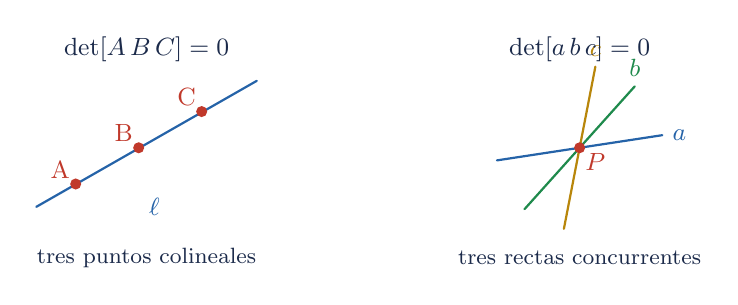
\begin{tikzpicture}[scale=1.0,>=Latex,line cap=round]
  % izquierda: 3 puntos colineales
  \begin{scope}
    \draw[azul,thick] (-0.3,-0.05) -- (2.5,1.55);
    \foreach \x/\y/\l in {0.2/0.24/A, 1.0/0.7/B, 1.8/1.16/C}{
      \fill[rojo] (\x,\y) circle (2pt);
      \node[rojo,above left=-2pt] at (\x,\y) {\small \l};
    }
    \node[azul] at (1.2,-0.05) {\small $\ell$};
    \node[navy] at (1.1,1.95) {\small $\det[A\,B\,C]=0$};
    \node[navy,font=\footnotesize] at (1.1,-0.7) {tres puntos colineales};
  \end{scope}
  % derecha: 3 rectas concurrentes
  \begin{scope}[xshift=5.6cm]
    \coordinate (P) at (1.0,0.7);
    \draw[azul,thick]  ($(P)+(-1.05,-0.16)$) -- ($(P)+(1.05,0.16)$) node[right]{\small $a$};
    \draw[verde,thick] ($(P)+(-0.7,-0.78)$)  -- ($(P)+(0.7,0.78)$)  node[above]{\small $b$};
    \draw[oro,thick]   ($(P)+(-0.2,-1.03)$)  -- ($(P)+(0.2,1.03)$)  node[above]{\small $c$};
    \fill[rojo] (P) circle (2pt);
    \node[rojo,below right=-2pt] at (P) {\small $P$};
    \node[navy] at (1.0,1.95) {\small $\det[a\,b\,c]=0$};
    \node[navy,font=\footnotesize] at (1.0,-0.7) {tres rectas concurrentes};
  \end{scope}
\end{tikzpicture}
\caption{Colinealidad de tres puntos (izquierda) y concurrencia de tres
rectas (derecha): enunciados duales gobernados por el mismo determinante.}
\label{fig:dual}
\end{figure}

\subsection{Pascal y Brianchon}

Otro par célebre: dos teoremas separados por casi dos siglos que la
dualidad muestra como uno solo. Comenzamos por el más antiguo.

\begin{teorema}
\textbf{Pascal (1640).} Si un hexágono está inscrito en una cónica, los
tres puntos de intersección de pares de lados opuestos son colineales.
\end{teorema}

\paragraph{Pasaje al dual.}
Como en Desargues, aplicamos $\delta$ término por término. Una
observación previa sobre las cónicas: una cónica no degenerada de
$\RP^2$ es \emph{autodual} —su dual via $\delta$ es la cónica formada
por sus rectas tangentes—. Así, ``cónica'' aparece en los dos lados; lo
que cambia es si la miramos como lugar de puntos (inscritos) o como
envolvente de rectas (circunscritas).

\begin{center}
\renewcommand{\arraystretch}{1.4}
\begin{tabular}{@{}p{0.18\textwidth}p{0.38\textwidth}p{0.38\textwidth}@{}}
\toprule
 & \textbf{Original (Pascal)} & \textbf{Dual ($\delta$) $=$ Brianchon} \\
\midrule
\textit{Figura} &
hexágono \textbf{inscrito} en una cónica (6~\textbf{puntos} sobre $\mathcal C$) &
hexágono \textbf{circunscrito} a una cónica (6~\textbf{rectas} tangentes a $\mathcal C$) \\
\textit{Elementos} &
sus 6 \textbf{lados} (rectas que unen vértices consecutivos) &
sus 6 \textbf{vértices} (puntos donde se cortan tangentes consecutivas) \\
\textit{Pares opuestos} &
3 pares de lados opuestos &
3 pares de vértices opuestos \\
\textit{Construcción} &
los \textbf{puntos} donde se cortan esos 3 pares &
las \textbf{rectas} que unen esos 3 pares (las ``diagonales principales'') \\
\textit{Conclusión} &
los 3 puntos son \emph{colineales} &
las 3 rectas son \emph{concurrentes} \\
\bottomrule
\end{tabular}
\end{center}

\noindent El enunciado de la columna derecha es, palabra por palabra, el
teorema que Charles-Julien Brianchon publicó en 1806:

\begin{teorema}
\textbf{Brianchon (1806) $=$ dual de Pascal.} Si un hexágono está
circunscrito a una cónica, las tres rectas que unen pares de vértices
opuestos concurren en un punto.
\end{teorema}

\noindent A diferencia de Desargues, aquí el dual \emph{no} es el
recíproco: Pascal y Brianchon son dos teoremas distintos, descubiertos
con $166$ años de diferencia. La dualidad muestra que el segundo es
gratis una vez probado el primero: una demostración de Pascal se traduce,
línea por línea bajo $\delta$, en una demostración de Brianchon. Ese es,
en concreto, el ``duplicar el conocimiento sin costo'' al que aludimos al
final del trabajo.

\subsection{El teorema de Desargues}
\label{sec:desargues}

Algunos teoremas son \textbf{autoduales}: coinciden con su propio dual. El
caso emblemático es el \textbf{teorema de Desargues}.

\begin{teorema}
Si dos triángulos $ABC$ y $A'B'C'$ son tales que las rectas $AA'$, $BB'$,
$CC'$ concurren en un punto $O$, entonces los tres puntos de intersección
de pares de lados correspondientes,
\[
  X=AB\cap A'B',\quad Y=BC\cap B'C',\quad Z=AC\cap A'C',
\]
son colineales (Figura~\ref*{fig:desargues}).
\end{teorema}

\begin{figure}[H]
\centering
\begin{tikzpicture}[scale=0.62,>=Latex,line cap=round]
  \coordinate (O)  at (0,0);
  \coordinate (A)  at (1.2,2.6);
  \coordinate (B)  at (2.8,1.0);
  \coordinate (C)  at (1.0,0.5);
  \coordinate (Ap) at ($(O)!1.75!(A)$);
  \coordinate (Bp) at ($(O)!1.55!(B)$);
  \coordinate (Cp) at ($(O)!2.3!(C)$);
  \foreach \p in {Ap,Bp,Cp}{ \draw[gris,dashed] (O) -- (\p); }
  \draw[azul,thick] (A)--(B)--(C)--cycle;
  \draw[rojo,thick] (Ap)--(Bp)--(Cp)--cycle;
  \coordinate (X) at (intersection of A--B and Ap--Bp);
  \coordinate (Y) at (intersection of B--C and Bp--Cp);
  \coordinate (Z) at (intersection of C--A and Cp--Ap);
  \draw[oro,thick] (X) -- (Z);
  \foreach \p in {X,Y,Z}{ \fill[oro] (\p) circle (1.8pt); }
  \node[oro] at ($(X)+(0.0,0.25)$) {\small $X$};
  \node[oro] at ($(Y)+(0.25,0.05)$) {\small $Y$};
  \node[oro] at ($(Z)+(-0.2,0.18)$) {\small $Z$};
  \foreach \p/\l/\pos in {O/O/below left, A/A/above left, B/B/below,
        C/C/below left, Ap/A'/above, Bp/B'/right, Cp/C'/left}{
    \fill[navy] (\p) circle (1.6pt);
    \node[navy,\pos=1pt,font=\footnotesize] at (\p) {$\l$};
  }
\end{tikzpicture}
\caption{Teorema de Desargues: dos triángulos en perspectiva desde $O$
tienen sus lados correspondientes cortándose en tres puntos colineales
$X,Y,Z$. Es un teorema autodual: su dual coincide con su recíproco.}
\label{fig:desargues}
\end{figure}

\paragraph{Pasaje al dual.}
Apliquemos la aplicación $\delta$ a la hipótesis y a la conclusión. Un
triángulo —tres puntos junto con sus tres rectas conectoras— es una figura
\emph{autodual}: al intercambiar puntos por rectas dentro del triángulo
se obtiene otro triángulo. Así, $\delta$ solo cambia las relaciones de
incidencia. Tradúzcase término por término:

\begin{center}
\renewcommand{\arraystretch}{1.4}
\begin{tabular}{@{}p{0.10\textwidth}p{0.40\textwidth}p{0.42\textwidth}@{}}
\toprule
 & \textbf{Original} & \textbf{Dual ($\delta$)} \\
\midrule
\textit{Hipótesis} &
las rectas $AA',\,BB',\,CC'$ \emph{concurren} en un \textbf{punto} $O$ &
los puntos $AB\cap A'B',\,BC\cap B'C',\,AC\cap A'C'$ son \emph{colineales} sobre una \textbf{recta} $o$ \\
\textit{Conclusión} &
los puntos $AB\cap A'B',\,BC\cap B'C',\,AC\cap A'C'$ son \emph{colineales} &
las rectas $AA',\,BB',\,CC'$ son \emph{concurrentes} \\
\bottomrule
\end{tabular}
\end{center}

\noindent En cada celda, $\delta$ hizo lo previsto: cambió ``recta'' por
``punto'', ``concurrente'' por ``colineal'' e intersección por unión.
Lo notable es que, al hacerlo, \emph{la hipótesis y la conclusión se
intercambiaron entre sí}.

\paragraph{Autodualidad como invarianza de un bicondicional.}
Si llamamos
\begin{align*}
  P\;&:\;\text{``$AA',\,BB',\,CC'$ concurren en un punto $O$''},\\
  \delta(P)\;&:\;\text{``$AB\!\cap\! A'B',\;BC\!\cap\! B'C',\;AC\!\cap\! A'C'$ son colineales sobre una recta $o$''},
\end{align*}
el teorema de Desargues completo —enunciado original más recíproco— es
exactamente el bicondicional
\[
  P \;\Longleftrightarrow\; \delta(P).
\]
Aplicar $\delta$ a toda la proposición, recordando que $\delta$ es
involución ($\delta\circ\delta=\mathrm{id}$), da
\[
  \delta(P) \;\Longleftrightarrow\; \delta(\delta(P))
  \;=\;
  \delta(P) \;\Longleftrightarrow\; P,
\]
que es \emph{el mismo enunciado}: solo se intercambian los dos lados del
$\Longleftrightarrow$. Esa invariancia bajo $\delta$ es lo que significa
que Desargues sea \textbf{autodual}. La demostración del teorema (a cargo
de otro expositor) cubre las dos direcciones del bicondicional a la vez.

\subsection{La dualidad como metateorema}

Vale la pena notar qué tipo de enunciado es este principio. No es un
teorema común: no nos dice un hecho sobre unos puntos y rectas concretos,
sino que afirma algo \emph{sobre los teoremas mismos}. Por eso se lo
describe como un \textbf{metateorema}: un teorema que habla de otros
teoremas.

Lo que dice, en concreto, es que cada vez que demostramos algo sobre
incidencia su versión dual queda demostrada automáticamente, sin hacer
ninguna cuenta nueva. La dualidad no nos da un resultado: nos
\emph{regala el doble} de resultados a la vez.

\paragraph{El mismo patrón en la lógica.}
La misma idea aparece en la lógica. Toda fórmula que sea siempre verdadera
y esté escrita con ``y'' ($\wedge$), ``o'' ($\vee$) y ``no'' ($\neg$)
sigue siendo siempre verdadera si intercambiamos $\wedge\leftrightarrow\vee$
y verdadero$\,\leftrightarrow\,$falso.

Su caso más conocido son las \textbf{leyes de De~Morgan}:
\[
  \neg(p\wedge q)\;\equiv\;\neg p\,\vee\,\neg q,
  \qquad
  \neg(p\vee q)\;\equiv\;\neg p\,\wedge\,\neg q.
\]
Son justamente las que hacen el intercambio: negar convierte cada ``y'' en
un ``o'' y viceversa.

El principio se extiende a la \emph{lógica de predicados}, donde alcanza a
los cuantificadores, $\forall\leftrightarrow\exists$:
\[
  \neg\,\forall x\,P(x)\;\equiv\;\exists x\,\neg P(x).
\]
Es decir: ``no todos cumplen'' equivale a ``existe alguno que no cumple''.

\paragraph{El mismo patrón en los conjuntos.}
Lo mismo ocurre con los conjuntos. Si en una identidad válida cambiamos la
unión $\cup$ por la intersección $\cap$ (y el conjunto total por el
vacío), obtenemos otra identidad válida. Otra vez son las leyes de
De~Morgan, ahora para conjuntos:
\[
  \overline{A\cup B}\;=\;\bar A\cap\bar B,
  \qquad
  \overline{A\cap B}\;=\;\bar A\cup\bar B.
\]

\paragraph{Por qué funciona en todos los casos.}
La razón común es simple: en cada uno los \textbf{axiomas de partida ya son
simétricos} respecto del intercambio de dos nociones —punto/recta,
``y''/``o'', $\cup$/$\cap$—. Si las reglas básicas no distinguen entre las
dos, nada de lo que se deduzca de ellas puede distinguirlas tampoco.

Así, la simetría de los axiomas se \emph{hereda} a todo el sistema, y los
teoremas salen automáticamente de a pares. No es casualidad que la tabla
anterior escriba \emph{unir} y \emph{cortar} como $\vee$ y $\wedge$: es la
misma estructura que ordena los conjuntos y las proposiciones de la
lógica.

% ======================================================================
\section{Homografías}
% ======================================================================
\label{sec:homografias}

Las transformaciones distinguidas de la geometría proyectiva del plano son
las \textbf{homografías} (también llamadas transformaciones proyectivas o
colineaciones).

\begin{defbox}
Una \textbf{homografía} $h:\RP^2\to\RP^2$ es una aplicación biyectiva
representada en coordenadas homogéneas por una matriz $3\times 3$
invertible $H$, definida salvo un factor escalar no nulo:
\[
  \lambda
  \begin{pmatrix} x'\\ y'\\ z'\end{pmatrix}
  \;=\;
  H \begin{pmatrix} x\\ y\\ z\end{pmatrix},
  \qquad
  H\in\mathrm{GL}_3(\R),
  \quad H\sim\mu H.
\]
\end{defbox}

\paragraph{¿Por qué $H\sim\mu H$? La misma proyectivización, ahora aplicada a matrices.}
La equivalencia entre $H$ y $\mu H$ no es una convención: es una
consecuencia inmediata de que la homografía actúa sobre clases —los
puntos de $\RP^2$ son ya vectores módulo escala—. Si reemplazamos $H$
por $\mu H$,
\[
  (\mu H)\,\mathbf{x} \;=\; \mu\,(H\mathbf{x}),
\]
y los vectores $H\mathbf{x}$ y $\mu H\mathbf{x}$ representan
\emph{el mismo punto} de $\RP^2$ (difieren solo por el factor $\mu$).
$H$ y $\mu H$ inducen, entonces, exactamente la misma transformación
sobre el plano proyectivo.

Visto desde más arriba, las matrices $3\times 3$ forman un espacio
vectorial $\R^{3\times 3}\cong\R^{9}$. La relación
$H\sim\mu H$ es \emph{la proyectivización de ese espacio}: el conjunto
de homografías es el espacio proyectivo $\mathbb P(\R^{9})\cong\RP^{8}$
restringido a matrices invertibles. Por eso $9$ entradas $-\,1$ escala
$=$ \textbf{8 grados de libertad}, y por eso bastan (y hacen falta)
cuatro pares punto--imagen en posición general para fijar una
homografía. Este grupo cociente se denota
\[
  \mathrm{PGL}_3(\R) \;=\; \mathrm{GL}_3(\R)\,\big/\,\R^{\times}.
\]

\paragraph{Las piezas del cociente.}
La igualdad anterior tiene cuatro símbolos:
\begin{itemize}[leftmargin=1.4em,itemsep=2pt]
\item \fbox{$\mathrm{GL}_3(\R)$} (\emph{general linear group}): el grupo
  de las \textbf{matrices reales $3\times 3$ invertibles}, con la
  multiplicación de matrices como operación. Es donde vive nuestra $H$.
\item \fbox{$\R^{\times}$}: el grupo \textbf{multiplicativo de los
  reales no nulos}, $\R\setminus\{0\}$ con la multiplicación. Es donde
  vive el factor $\mu\neq 0$ por el que multiplicamos $H$.
\item \fbox{$\mathrm{GL}_3(\R)/\R^{\times}$}: el cociente que
  \textbf{identifica matrices que difieren por un escalar}, es decir,
  $H$ y $\mu H$. Implementa exactamente la equivalencia $H\sim\mu H$ a
  nivel de grupo.
\item \fbox{$\mathrm{PGL}_3(\R)$} (\emph{projective general linear
  group}): \textbf{el grupo de homografías de $\RP^{2}$}. Una sutileza
  tipográfica: el subíndice $3$ es el tamaño de la matriz, no la
  dimensión del espacio proyectivo — $\mathrm{PGL}_3(\R)$ actúa sobre
  $\RP^{3-1}=\RP^{2}$—. En general, $\mathrm{PGL}_{n+1}(\R)$ es el
  grupo de homografías de $\RP^{n}$.
\end{itemize}

\paragraph{Un ejemplo concreto.}
Consideremos la homografía dada por
\[
  H \;=\;
  \begin{pmatrix}
    1 & 0 & 0\\
    0 & 1 & 0\\
    1 & 0 & 1
  \end{pmatrix}.
\]
Veamos cómo actúa sobre tres puntos representativos de $\RP^2$,
recordando que después de multiplicar por $H$ hay que normalizar
($\div z$) para volver al plano afín:
\begin{center}
\renewcommand{\arraystretch}{1.35}
\begin{tabular}{@{}lll@{}}
\toprule
$P=\hp{x}{y}{z}$ (afín) & $H\cdot P$ (homogéneo) & punto resultado (afín) \\
\midrule
$\hp{0}{0}{1}=(0,0)$ & $\hp{0}{0}{1}$ & $(0,0)$ \quad\text{(fijo)} \\
$\hp{1}{0}{1}=(1,0)$ & $\hp{1}{0}{2}$ & $(1/2,\,0)$ \\
$\hp{2}{0}{1}=(2,0)$ & $\hp{2}{0}{3}$ & $(2/3,\,0)$ \\
$\hp{1}{0}{0}=\infty_x$ & $\hp{1}{0}{1}$ & $(1,\,0)$ \\
\bottomrule
\end{tabular}
\end{center}

\noindent Las dos cosas notables del ejemplo:
\begin{itemize}[leftmargin=1.4em,itemsep=2pt]
\item los puntos del eje $x$ se acumulan: $(1,0)\mapsto(1/2,0)$,
  $(2,0)\mapsto(2/3,0)$, $(3,0)\mapsto(3/4,0)$, $\ldots$ — toda la
  semirrecta positiva se aplasta dentro de $(0,1)$;
\item el \textbf{punto al infinito} de la dirección $x$, $\hp{1}{0}{0}$,
  pasa a $\hp{1}{0}{1}=(1,0)$, que es un \textbf{punto finito}.
\end{itemize}
Esta segunda propiedad es la firma de una homografía propiamente
proyectiva: ninguna aplicación afín ($z'=z$, última fila $(0,0,1)$)
puede llevar un punto al infinito a uno finito. Es exactamente lo que
hace falta en aplicaciones como la \emph{rectificación de documentos}
de la Sección~\ref{sec:vision-homografia}: enderezar la perspectiva
significa mandar a distancia finita el punto de fuga donde concurrían
los bordes paralelos.

\paragraph{Qué preservan las homografías.}
Colinealidad, concurrencia, incidencia y la \emph{razón doble}
(cross-ratio) de cuatro puntos alineados. \textbf{No} preservan
distancias, ángulos ni razones simples; tampoco el paralelismo (que en
$\RP^2$ ni siquiera existe como noción intrínseca: dos rectas siempre
se cortan).

El siguiente teorema (Santaló, §9.5) justifica que las homografías son
\emph{las} transformaciones de la geometría proyectiva del plano real.

\begin{teorema}
Toda colineación de $\RP^2$ —es decir, toda biyección que aplica puntos
alineados en puntos alineados— es una homografía.
\end{teorema}

% ======================================================================
\section{Aplicaciones e importancia}
% ======================================================================

\subsection{Perspectiva y arte}

El origen mismo de la disciplina. La Figura~\ref{fig:persp}, que ya
discutimos como ilustración de la carta afín, ofrece también la lectura
artística: cuando un pintor dibuja rieles o un piso que se aleja, las
rectas paralelas convergen hacia un \textbf{punto de fuga} sobre la línea
del horizonte. Ese punto y esa línea son, literalmente, un punto al
infinito y la recta del infinito de $\RP^2$.

\subsection{El modelo de cámara estenopeica}
\label{sec:camera}

El esquema más simple de una cámara —el \emph{pinhole}— captura cómo un
sensor plano forma la imagen del mundo. Un punto del mundo
$\mathbf{X}=(X,Y,Z)$, un agujero infinitesimal $O$ y un plano imagen
detrás de él determinan, mediante una proyección lineal, un punto
$(u,v)$ del sensor. En coordenadas homogéneas todo el modelo se expresa
con una sola ecuación.

\begin{teorema}
\centering\large
$\displaystyle \lambda
\begin{pmatrix} u\\ v\\ 1\end{pmatrix}
=
\underbrace{K}_{3\times 3}
\;
\underbrace{[\,R\mid t\,]}_{3\times 4}
\begin{pmatrix} X\\ Y\\ Z\\ 1\end{pmatrix}.$
\end{teorema}

\paragraph{¿Por qué el punto del mundo tiene cuatro entradas?}
A primera vista llama la atención que el vector de entrada
$[X:Y:Z:1]$ tenga cuatro componentes si estamos describiendo un punto
de $\R^3$. La regla es la misma de antes, ahora subida una dimensión:
\emph{el espacio proyectivo $\RP^n$ se construye proyectivizando
$\R^{n+1}$, así que un punto de $\RP^n$ tiene siempre $n+1$ coordenadas
homogéneas}. Como el mundo es tridimensional, lo proyectivizamos a
$\RP^3$, y por eso aparecen cuatro componentes. Y como
$\hpf{X}{Y}{Z}{1}$ y $\hpf{X}{Y}{Z}{0}$ representan cosas muy distintas,
escribir el ``$1$'' al final no es trivial:
\[
  \underbrace{(X,Y,Z)\in\R^3}_{\text{punto afín}}
  \;\hookrightarrow\;
  \underbrace{\hpf{X}{Y}{Z}{1}\in\RP^{3}}_{\text{misma posición, carta afín }W=1}
  \qquad\text{vs.}\qquad
  \underbrace{\hpf{X}{Y}{Z}{0}\in\RP^{3}}_{\text{dirección, punto al infinito}}.
\]
La inmersión $\R^3\hookrightarrow\RP^3$ por $(X,Y,Z)\mapsto\hpf{X}{Y}{Z}{1}$
es la versión 3D de la que usamos al principio para $\R^2\hookrightarrow\RP^2$.

Esta subida de dimensión no es cosmética: es lo que vuelve
\textbf{lineal} a toda la cámara. La proyección $\R^3\to\R^2$ del mundo
al sensor implica dividir por la profundidad $Z$ —una operación
\emph{no} lineal—. Pero el modelo proyectivo
\[
  \R^3 \;\hookrightarrow\; \RP^{3}
  \;\xrightarrow{\;K[R\mid t]\;}\; \RP^{2}
  \;\twoheadrightarrow\; \R^{2}
\]
oculta esa división en el último paso (la carta afín $\div w'$): toda
la geometría intermedia es \emph{una sola multiplicación de matrices}.

\paragraph{Los tres factores.}
\begin{itemize}[leftmargin=1.2em,itemsep=2pt]
\item $K\in\R^{3\times 3}$ —la matriz de \emph{intrínsecos}— codifica las
  propiedades internas de la cámara: distancia focal y centro óptico
  (píxeles por unidad de longitud).
\item $[R\mid t]\in\R^{3\times 4}$ —los \emph{extrínsecos}— describe la
  pose: una rotación $R$ y una traslación $t$ que llevan el sistema de
  referencia del mundo al de la cámara. Tiene $3$ filas y $4$ columnas
  porque convierte un punto de $\RP^3$ (entrada de $4$ componentes) en
  uno de la cámara, $\RP^2$ todavía no normalizado (salida de $3$).
\item $\lambda\neq0$ es el factor proyectivo: dividir por $\lambda$ al
  final \emph{es} la conversión homogéneo $\to$ afín
  $\hp{u'}{v'}{w'}\mapsto(u'/w',v'/w')$ de la
  Sección~\ref{sec:carta}, y no un truco numérico.
\end{itemize}

\begin{figure}[ht]
\centering
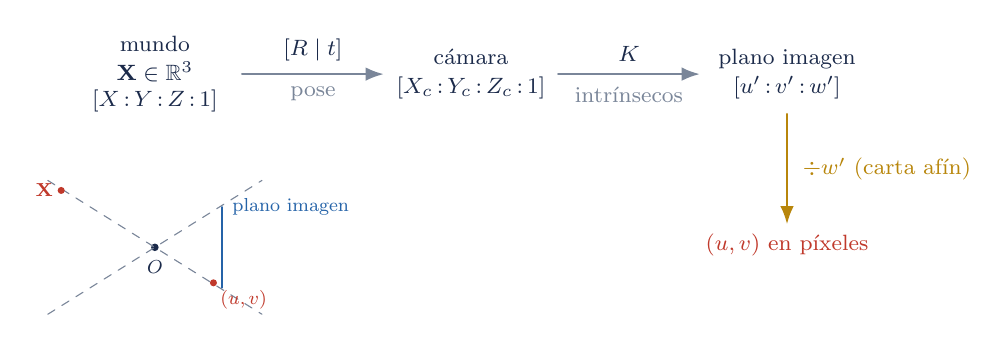
\begin{tikzpicture}[
    >=Latex,line cap=round,
    box/.style={navy,align=center,font=\footnotesize,
                inner sep=3pt,minimum height=10mm,minimum width=22mm},
    title/.style={navy,font=\footnotesize\itshape,gris},
    arr/.style={->,gris,thick},
    arrlab/.style={navy,font=\footnotesize},
    arrlow/.style={gris,font=\footnotesize}]
  % --- fila superior: chain mundo -> cámara -> plano imagen
  \node[box] (mundo)
    {mundo\\[1pt]$\mathbf{X}\in\R^3$\\\footnotesize$\hpf{X}{Y}{Z}{1}$};
  \node[box,right=18mm of mundo] (cam)
    {cámara\\[1pt]$\hpf{X_c}{Y_c}{Z_c}{1}$};
  \node[box,right=18mm of cam] (img)
    {plano imagen\\[1pt]$\hp{u'}{v'}{w'}$};
  % flechas con etiquetas
  \draw[arr] (mundo) -- (cam)
        node[midway,above=1pt,arrlab]{$[R\mid t]$}
        node[midway,below=1pt,arrlow]{pose};
  \draw[arr] (cam) -- (img)
        node[midway,above=1pt,arrlab]{$K$}
        node[midway,below=1pt,arrlow]{intrínsecos};
  % perspective divide hacia abajo
  \node[rojo,font=\footnotesize,below=14mm of img] (px) {$(u,v)$ en píxeles};
  \draw[->,oro,thick] (img) -- (px)
        node[midway,right=2pt,oro,font=\footnotesize]{$\div w'$ (carta afín)};
  % esquema pinhole compacto a la izquierda-abajo
  \begin{scope}[xshift=0mm,yshift=-22mm,scale=0.85,every node/.style={transform shape}]
    \fill[navy] (0,0) circle (1.6pt);
    \node[navy,font=\footnotesize,below] at (0,-0.08) {$O$};
    \draw[gris,dashed] (-1.6,1.0) -- (0,0) -- (1.6,-1.0);
    \draw[gris,dashed] (-1.6,-1.0) -- (0,0) -- (1.6,1.0);
    \draw[azul,thick] (1.0,-0.6) -- (1.0,0.6);
    \node[azul,font=\footnotesize,right=1pt] at (1.0,0.6) {plano imagen};
    \fill[rojo] (-1.4,0.85) circle (1.5pt);
    \node[rojo,font=\footnotesize,left] at (-1.4,0.85) {$\mathbf{X}$};
    \fill[rojo] (0.875,-0.53) circle (1.5pt);
    \node[rojo,font=\footnotesize,below right=-1pt] at (0.88,-0.55) {$(u,v)$};
  \end{scope}
\end{tikzpicture}
\caption{Modelo de cámara estenopeica. Los extrínsecos $[R\mid t]$ llevan
el mundo al sistema de la cámara; los intrínsecos $K$ proyectan al plano
imagen homogéneo; la división por $w'$ recupera las coordenadas en
píxeles. El esquema inferior izquierdo recuerda la geometría: un rayo por
el agujero $O$ del mundo al plano imagen.}
\label{fig:pinhole}
\end{figure}

Esta es una de las identidades centrales de la visión por computadora: una
ecuación lineal sobre coordenadas homogéneas que esconde, en su
interior, una proyección no lineal. Toda la maquinaria —calibración,
reconstrucción 3D, fusión LiDAR--cámara— se monta sobre ella.

\paragraph{Un ejemplo numérico realista.}
Supongamos una cámara con sensor de $1280\times 720$ píxeles, distancia
focal equivalente a $1000$ píxeles y centro óptico en el medio de la
imagen. Sus intrínsecos son
\[
  K \;=\;
  \begin{pmatrix}
    1000 & 0 & 640 \\
    0 & 1000 & 360 \\
    0 & 0 & 1
  \end{pmatrix}.
\]

\paragraph{¿De dónde salen los dos $1000$, y qué es la distancia focal?}
La forma general de los intrínsecos es
\[
  K \;=\;
  \begin{pmatrix}
    f_x & 0 & c_x \\
    0 & f_y & c_y \\
    0 & 0 & 1
  \end{pmatrix},
\]
donde $(c_x,c_y)$ es el centro óptico —aquí la mitad del sensor,
$(640,360)$— y los dos números de la diagonal, $f_x$ y $f_y$, son la
\emph{distancia focal expresada en píxeles}. Aparece dos veces porque la
proyección actúa por separado sobre el eje horizontal ($x$) y el vertical
($y$); en una cámara con píxeles cuadrados ambos coinciden,
$f_x=f_y=1000$, y solo serían distintos si los píxeles fuesen
rectangulares.

La distancia focal mide \emph{cuánto amplía} la cámara la escena al
proyectarla sobre el sensor. La proyección de un punto $3$D en
coordenadas de la cámara $(X,Y,Z)$ a un píxel es
\[
  u \;=\; f_x\,\frac{X}{Z} + c_x,
  \qquad
  v \;=\; f_y\,\frac{Y}{Z} + c_y .
\]
El cociente $X/Z$ es solo un \emph{ángulo} (una proporción sin unidades);
para convertirlo en píxeles hace falta un factor de escala, y ese factor
\emph{es} la distancia focal en píxeles. Por eso $f$ va en píxeles y no en
milímetros. Su relación con la focal física de la lente es
\[
  f_{\text{px}} \;=\; \frac{f_{\text{mm}}}{\text{tamaño de un píxel en mm}} .
\]
Por ejemplo, con píxeles de $4\,\mu\text{m} = 0{,}004$~mm y una lente de
$4$~mm se obtiene $f_{\text{px}} = 4/0{,}004 = 1000$~píxeles, justo el
valor de este ejemplo. Intuitivamente, $f=1000$~px significa que un
objeto situado a una distancia $Z$ igual a su propio tamaño ocuparía
$1000$~píxeles en la imagen: cuanto mayor es $f$, más «teleobjetivo»
(más zoom, menor campo de visión); cuanto menor, más gran angular.

La cámara va montada $1$ metro a la derecha del centro del vehículo y
mira hacia adelante (sin rotación respecto del sistema del auto). Como
el origen del mundo lo ponemos en el centro del vehículo, los
extrínsecos son
\[
  R \;=\; I_{3} \;=\;
  \begin{pmatrix} 1 & 0 & 0 \\ 0 & 1 & 0 \\ 0 & 0 & 1 \end{pmatrix},
  \qquad
  t \;=\;
  \begin{pmatrix} -1 \\ 0 \\ 0 \end{pmatrix}
  \;\text{(metros).}
\]
El signo negativo de $t$ se debe a que $[R\mid t]$ lleva del mundo a la
cámara: para que un punto en la posición de la cámara
($X_w=(1,0,0)$) caiga en el origen del sistema-cámara, hace falta
restar $1$ a la coordenada~$x$.

Tomemos un peatón a $10$~metros adelante del auto, alineado con el
centro del vehículo: $X_w = (0,\,0,\,10)$. La cadena completa es:
\begin{enumerate}[leftmargin=1.4em,itemsep=2pt]
\item \textbf{Mundo $\to$ cámara} (extrínsecos):
\[
  [R\mid t]\!
  \begin{pmatrix} 0\\ 0\\ 10\\ 1\end{pmatrix}
  =
  R\!\begin{pmatrix} 0\\0\\10\end{pmatrix} + t
  = \begin{pmatrix} 0\\0\\10\end{pmatrix} + \begin{pmatrix} -1\\0\\0\end{pmatrix}
  = \begin{pmatrix} -1\\ 0\\ 10\end{pmatrix}.
\]
El peatón aparece, en el sistema de la cámara, $1$~m a la izquierda y
$10$~m adelante.
\item \textbf{Cámara $\to$ plano imagen homogéneo} (intrínsecos):
\[
  K\!\begin{pmatrix} -1\\ 0\\ 10\end{pmatrix}
  =
  \begin{pmatrix}
    1000\cdot(-1)+0\cdot 0+640\cdot 10\\
    0\cdot(-1)+1000\cdot 0+360\cdot 10\\
    10
  \end{pmatrix}
  =
  \begin{pmatrix} 5400\\ 3600\\ 10\end{pmatrix}.
\]
\item \textbf{Carta afín} (división por $w'=10$):
\[
  (u,v) \;=\; \left(\tfrac{5400}{10},\,\tfrac{3600}{10}\right)
  \;=\; (540,\,360).
\]
\end{enumerate}
El peatón aparece en el píxel $(540,360)$: a la altura vertical del
centro de la imagen ($360$, como esperábamos, porque está al mismo
nivel) y $100$~px a la izquierda del centro horizontal ($640-540=100$).
La cuenta concuerda con la intuición: el peatón está a $1$~m a la
izquierda visto desde una cámara que ``mide'' a $10$~m, y el ángulo
$\tan^{-1}(1/10)$ se traduce, multiplicado por la focal de $1000$ px,
exactamente en $100$ píxeles de desplazamiento.

Si en lugar del peatón hubiéramos pasado el \textbf{punto al infinito} de
la dirección $z$, $\hpf{0}{0}{1}{0}$ —que representa ``infinitamente
lejos hacia adelante''—, el cálculo daría
$K[R\mid t]\hpf{0}{0}{1}{0}^\top = K(0,0,1)^\top = (640,360,1)^\top$,
o sea exactamente el píxel del centro de la imagen: el \emph{punto de
fuga} de la dirección de marcha.

\begin{figure}[H]
\centering
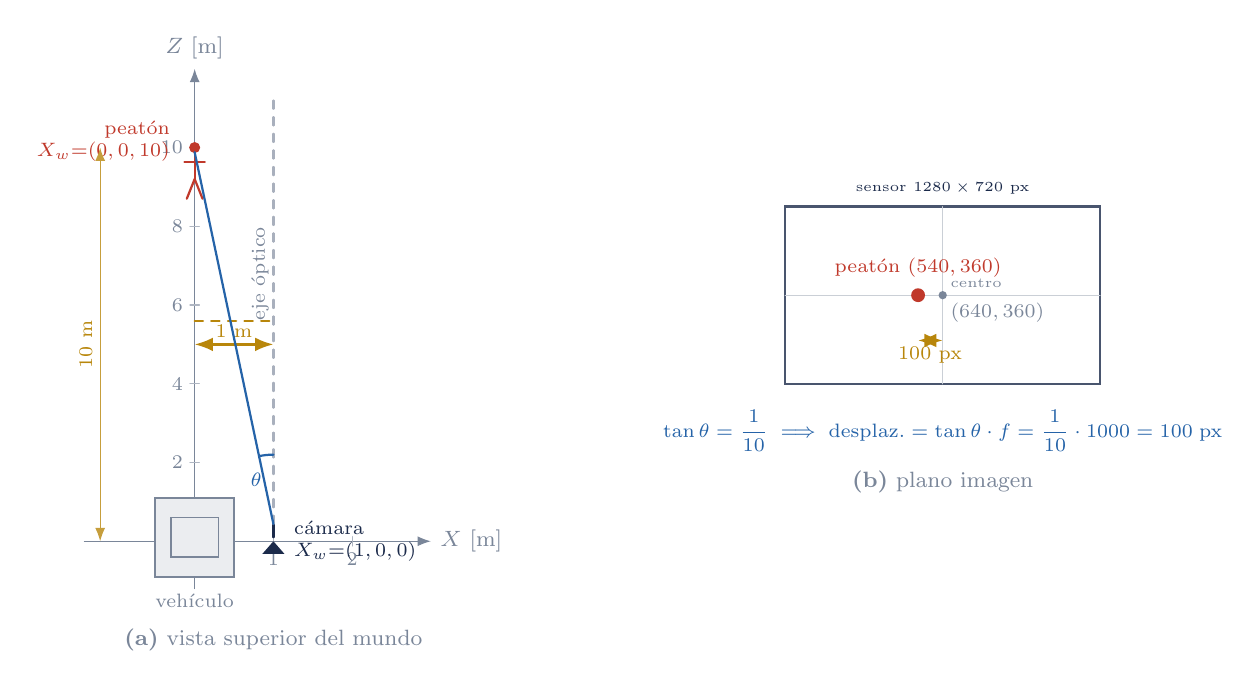
\begin{tikzpicture}[>=Latex,line cap=round]

  % ==================================================
  % PANEL A — vista superior del mundo (plano XZ)
  % ==================================================
  \begin{scope}
    % Ejes
    \draw[->,gris] (-1.4,0) -- (3.0,0) node[right,gris,font=\footnotesize]{$X$ [m]};
    \draw[->,gris] (0,-0.6) -- (0,6.0) node[above,gris,font=\footnotesize]{$Z$ [m]};
    \node[gris,font=\scriptsize,below left=-2pt] at (0,0) {$O_w$};
    % marcas en X
    \foreach \x in {1,2}{
      \draw[gris!60] (\x,-0.06) -- (\x,0.06);
      \node[gris,font=\scriptsize,below=-1pt] at (\x,-0.06) {\x};
    }
    % marcas en Z (escala 1 unidad = 2 m)
    \foreach \z in {1,2,3,4,5}{
      \draw[gris!60] (-0.06,\z) -- (0.06,\z);
      \pgfmathtruncatemacro{\zm}{\z*2}
      \node[gris,font=\scriptsize,left=-1pt] at (-0.06,\z) {\zm};
    }

    % --- Vehículo (rectángulo con techo)
    \fill[gris!15]   (-0.5,-0.45) rectangle (0.5,0.55);
    \draw[gris,thick] (-0.5,-0.45) rectangle (0.5,0.55);
    \draw[gris,thin]  (-0.3,-0.2)  rectangle (0.3,0.30);
    \node[gris,font=\scriptsize] at (0,-0.75) {vehículo};

    % --- Cámara (triangulito apuntando +Z) sobre el techo del vehículo
    \fill[navy] (1,0.0) -- (0.86,-0.16) -- (1.14,-0.16) -- cycle;
    \draw[navy,thick] (1,0.05) -- (1,0.22);
    \node[navy,font=\scriptsize,right=4pt,align=left]
          at (1.0,0.0) {cámara\\$X_w{=}(1,0,0)$};

    % --- Eje óptico (línea de puntos hacia adelante)
    \draw[gris!65,dashed,thick] (1,0.22) -- (1,5.7);
    \node[gris,font=\scriptsize,rotate=90] at (0.83,3.4) {eje óptico};

    % --- Peatón (figurita simple)
    \fill[rojo] (0,5) circle (2pt); % cabeza
    \draw[rojo,thick] (0,4.94) -- (0,4.6); % torso
    \draw[rojo,thick] (-0.13,4.82) -- (0.13,4.82); % brazos
    \draw[rojo,thick] (0,4.6) -- (-0.1,4.35); % piernas
    \draw[rojo,thick] (0,4.6) -- (0.1,4.35);
    \node[rojo,font=\scriptsize,left=4pt,align=right]
          at (-0.05,5.08) {peatón\\$X_w{=}(0,0,10)$};

    % --- Distancia transversal 1 m (a mitad de altura, bien visible)
    \draw[oro,thick,dashed] (0,2.8) -- (1,2.8);
    \draw[oro,thick,<->]    (0,2.5) -- (1,2.5);
    \node[oro,font=\scriptsize,above=-1pt] at (0.5,2.5) {$1$ m};

    % --- Distancia longitudinal 10 m a la izquierda
    \draw[oro!80,thin,<->] (-1.2,0.0) -- (-1.2,5.0);
    \node[oro,font=\scriptsize,rotate=90] at (-1.38,2.5) {$10$ m};

    % --- Rayo cámara → peatón
    \draw[azul,thick] (1,0.22) -- (0,4.94);

    % --- Ángulo θ
    \draw[azul,thick] (1,1.10) arc[start angle=90,end angle=101.6,radius=0.88];
    \node[azul] at (0.78,0.78) {\scriptsize $\theta$};

    % --- Título del panel
    \node[gris,font=\footnotesize] at (1.0,-1.25)
          {\textbf{(a)} vista superior del mundo};
  \end{scope}

  % ==================================================
  % PANEL B — plano imagen (píxeles)
  % ==================================================
  \begin{scope}[xshift=7.5cm,yshift=2.0cm]
    % Marco del sensor
    \draw[navy!80,thick] (0,0) rectangle (4.0,2.25);
    \node[navy,font=\tiny,above=1pt] at (2,2.25) {sensor $1280\times720$ px};

    % Cruz central
    \draw[gris!40] (2,0) -- (2,2.25);
    \draw[gris!40] (0,1.125) -- (4,1.125);

    % Centro óptico
    \fill[gris] (2,1.125) circle (1.5pt);
    \node[gris,font=\scriptsize,below right=-1pt] at (2,1.125) {$(640,360)$};
    \node[gris,font=\tiny,above right=-1pt] at (2,1.125) {centro};

    % Peatón en el plano imagen (540, 360) → (1.6875, 1.125)
    \fill[rojo] (1.6875,1.125) circle (2.5pt);
    \node[rojo,font=\scriptsize,above=3pt] at (1.6875,1.125)
          {peatón $(540,360)$};

    % Flecha de los 100 px de desfasaje
    \draw[oro,thick,<->] (1.6875,0.55) -- (2.0,0.55);
    \node[oro,font=\scriptsize,below=-1pt] at (1.84,0.55) {$100$ px};

    % Anotación con la cuenta del ángulo
    \node[azul,font=\scriptsize,align=center] at (2,-0.6)
          {$\tan\theta=\dfrac{1}{10}
            \;\Longrightarrow\;
            \text{desplaz.}=\tan\theta\cdot f
            =\dfrac{1}{10}\cdot 1000=100\;\text{px}$};

    % Título
    \node[gris,font=\footnotesize] at (2,-1.25)
          {\textbf{(b)} plano imagen};
  \end{scope}
\end{tikzpicture}
\caption{Dos vistas del ejemplo numérico. \textbf{(a)} Vista superior
del mundo: el vehículo está en el origen $O_w$, la cámara a $1$~m a la
derecha mirando hacia $+Z$, el peatón $10$~m adelante alineado con el
centro del vehículo. El rayo cámara--peatón forma con el eje óptico un
ángulo $\theta$ con $\tan\theta=1/10$. (El eje $Z$ está comprimido $1{:}2$
para que la figura quepa en la página.) \textbf{(b)} Resultado en el
plano imagen: el peatón aparece en el píxel $(540,360)$, a $100$ píxeles
a la izquierda del centro óptico $(640,360)$. La cuenta cierra:
$\tan\theta\cdot f = \tfrac{1}{10}\cdot 1000 = 100$ px.}
\label{fig:pinhole-numexample}
\end{figure}

\subsection{Visión por computadora: homografías de planos}
\label{sec:vision-homografia}

La Sección~\ref{sec:homografias} introdujo las homografías de modo
abstracto; aquí aparecen en dos problemas cotidianos.

\paragraph{Panorámicas (\emph{image stitching}).}
Si una cámara solo \emph{rota} alrededor de su centro óptico (sin
trasladarse), las dos vistas del mismo plano del mundo se relacionan
exactamente por una homografía. Para construir un panorama el sistema:
\begin{enumerate}[leftmargin=1.4em,itemsep=2pt]
\item detecta puntos de interés y empareja correspondencias;
\item estima la homografía $H$ que mejor alinea ambas imágenes (basta con
  cuatro pares en posición general);
\item aplica $H$ para deformar (\emph{warpear}) una imagen sobre la otra y
  obtiene la imagen unificada.
\end{enumerate}

La intuición proyectiva es la siguiente: cada foto es una \emph{vista}
distinta de la misma escena, todas tomadas desde el mismo centro óptico,
así que son representaciones proyectivas relacionadas entre sí. Como el
centro de proyección es común, las diferencias entre fotos consecutivas no
dependen de la profundidad de la escena, sino solo del giro de la cámara,
y por eso se capturan exactamente con una homografía. El algoritmo elige
una imagen como \textbf{marco de referencia} y busca las homografías que
llevan a las demás a ese mismo plano imagen; una vez alineadas todas en
ese marco común, se mezclan en una sola foto panorámica
(Figura~\ref{fig:panorama}). No se unifica un «punto», sino el sistema de
coordenadas del plano sobre el que se proyecta todo.

\begin{figure}[H]
\centering
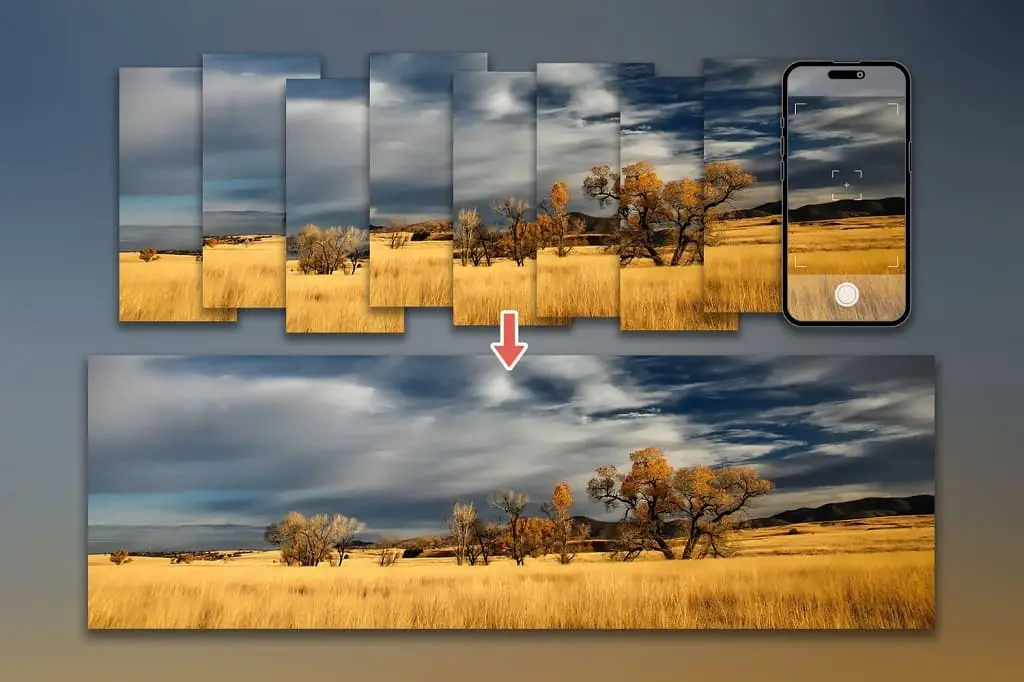
\includegraphics[width=0.82\linewidth]{figuras/panorama_stitching.png}
\caption{\emph{Image stitching}: varias fotos tomadas girando la cámara
  sobre su centro óptico (arriba) son vistas proyectivas de la misma
  escena. El algoritmo estima la homografía que alinea cada una con un
  marco de referencia común y las fusiona en una única panorámica
  (abajo).}
\label{fig:panorama}
\end{figure}

\paragraph{Rectificación de documentos.}
Una foto de un documento tomada en ángulo aparece como un cuadrilátero
deformado. Detectadas las cuatro esquinas $P_1,\dots,P_4$ y elegido un
rectángulo objetivo $Q_1,\dots,Q_4$, hay una única homografía $H$ con
$H\,P_i = Q_i$; aplicar $H^{-1}$ al pixel-grid produce la imagen frontal
sin deformación perspectiva. Es el algoritmo que está detrás de los
escáneres móviles (CamScanner, Adobe Scan, Apple Notes,\ldots), como se
ve en la Figura~\ref{fig:camscanner}.

\begin{figure}[H]
\centering
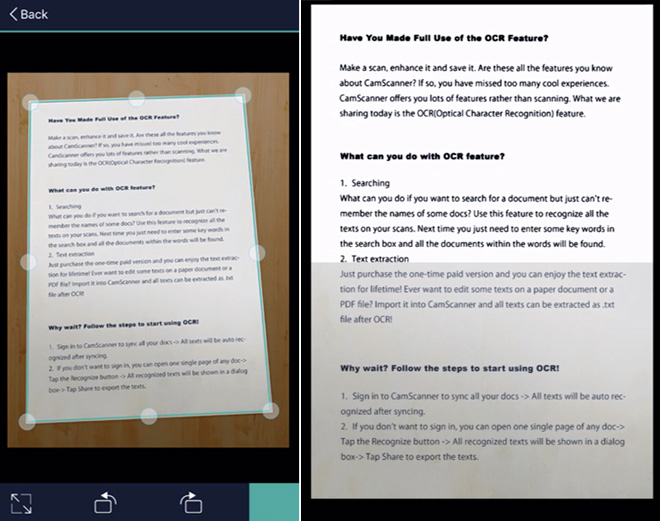
\includegraphics[width=0.72\linewidth]{figuras/escaneo_camscanner.png}
\caption{Escaneo de documentos en CamScanner. \emph{Izquierda:} la foto
  tomada en ángulo; el documento aparece como un cuadrilátero cuyos
  bordes —paralelos en el papel real— se ven \emph{convergiendo} hacia un
  punto de fuga por efecto de la perspectiva. \emph{Derecha:} tras
  aplicar la homografía de rectificación, el documento se ve frontal y
  rectangular.}
\label{fig:camscanner}
\end{figure}

\paragraph{Una lectura proyectiva: restaurar el paralelismo.}
Conviene aclarar un punto fino, porque es tentador pensar que la
homografía «preserva» las rectas paralelas: en general \emph{no} lo hace
—esa es precisamente la diferencia entre la geometría proyectiva y la
afín—. Lo que ocurre aquí es lo contrario. Los bordes del documento son
paralelos en el papel, pero la cámara, que es una transformación
proyectiva, los proyecta como rectas que \emph{convergen} hacia un punto
de fuga: un punto al infinito que se volvió finito en la imagen. La
homografía de rectificación $H^{-1}$ hace el camino inverso, enviando ese
punto de fuga de regreso a la recta del infinito; al hacerlo, los bordes
recuperan el paralelismo y el documento se ve de frente. En el lenguaje
de las Secciones anteriores: rectificar es elegir la homografía que
manda el punto de fuga de los bordes del documento de vuelta al infinito,
es decir, que \emph{restaura} —no que preserva— el paralelismo.

\begin{figure}[H]
\centering
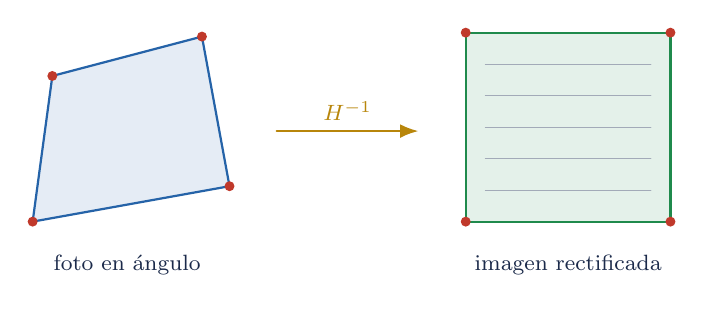
\begin{tikzpicture}[scale=1.0,>=Latex,line cap=round]
  % cuadrilatero deformado
  \begin{scope}
    \coordinate (P1) at (0.1,0.0);
    \coordinate (P2) at (2.6,0.45);
    \coordinate (P3) at (2.25,2.35);
    \coordinate (P4) at (0.35,1.85);
    \fill[azul!12] (P1)--(P2)--(P3)--(P4)--cycle;
    \draw[azul,thick] (P1)--(P2)--(P3)--(P4)--cycle;
    \foreach \p in {P1,P2,P3,P4}{ \fill[rojo] (\p) circle (1.8pt); }
    \node[navy,font=\footnotesize] at (1.3,-0.55) {foto en ángulo};
  \end{scope}
  % flecha H^{-1}
  \draw[->,oro,thick] (3.2,1.15) -- (5.0,1.15)
        node[midway,above,font=\footnotesize,oro]{$H^{-1}$};
  % rectangulo rectificado
  \begin{scope}[xshift=5.6cm]
    \coordinate (Q1) at (0,0);
    \coordinate (Q2) at (2.6,0);
    \coordinate (Q3) at (2.6,2.4);
    \coordinate (Q4) at (0,2.4);
    \fill[verde!12] (Q1)--(Q2)--(Q3)--(Q4)--cycle;
    \draw[verde,thick] (Q1)--(Q2)--(Q3)--(Q4)--cycle;
    \foreach \p in {Q1,Q2,Q3,Q4}{ \fill[rojo] (\p) circle (1.8pt); }
    % filas de "texto"
    \foreach \y in {0.4,0.8,1.2,1.6,2.0}{
      \draw[gris!70,thin] (0.25,\y) -- (2.35,\y);
    }
    \node[navy,font=\footnotesize] at (1.3,-0.55) {imagen rectificada};
  \end{scope}
\end{tikzpicture}
\caption{Rectificación por homografía: las cuatro esquinas detectadas en la
foto deformada se llevan a las esquinas de un rectángulo objetivo; la
homografía $H$ queda determinada por esas cuatro correspondencias.}
\label{fig:rectif}
\end{figure}

\subsection{Gráficos por computadora: el \emph{pipeline} de la GPU}

\paragraph{Qué es, en el fondo, un modelo 3D.}
Antes de hablar de matrices conviene ver qué se está transformando. Un
modelo 3D —un personaje, un auto, el conejo de la
Figura~\ref{fig:malla}— no es una superficie continua: es una
\emph{malla} (\emph{mesh}), es decir, una colección finita de
\textbf{vértices} (puntos $(X,Y,Z)$) unidos en \textbf{triángulos}. Cada
triángulo aproxima un trozo plano de la superficie, y al pegar muchos se
reconstruye la forma curva. Cuantos más triángulos, más fiel es la
aproximación: en la Figura~\ref{fig:malla} el mismo conejo aparece con un
número creciente de caras, desde una versión tosca y facetada hasta una
casi lisa.

\begin{figure}[h]
  \centering
  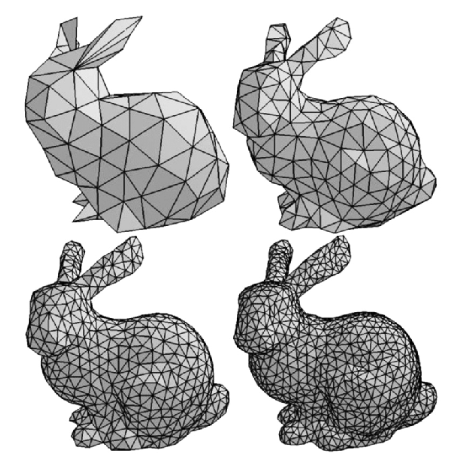
\includegraphics[width=0.6\linewidth]{figuras/malla_conejo.png}
  \caption{El \emph{conejo de Stanford} representado como malla de
    triángulos con resolución creciente. La superficie no se almacena de
    forma continua, sino como una nube de vértices conectados en caras
    triangulares; a mayor cantidad de triángulos, mejor se aproxima la
    forma real. Animar o mover el modelo consiste en aplicar a esos
    vértices las transformaciones lineales de las que trata esta sección.}
  \label{fig:malla}
\end{figure}

La clave para lo que sigue es que \emph{toda la geometría del modelo vive
en sus vértices}. Mover el objeto, rotarlo, escalarlo, simular cómo lo
empuja una fuerza o cómo cae por gravedad —las reglas de la física del
mundo virtual— se reduce, al final del cálculo, a \textbf{transformar las
coordenadas de cada vértice}. Y como veremos, en coordenadas homogéneas
todas esas transformaciones se expresan de manera uniforme como una sola
multiplicación matricial, lo que permite a la GPU procesar millones de
vértices en paralelo.

En gráficos por computadora cada vértice $(X,Y,Z)$ de la escena se
representa como un vector $\hpf{X}{Y}{Z}{1}$ y todas las transformaciones
—traslación, rotación, escala, proyección en perspectiva— se unifican como
multiplicaciones por matrices $4\times 4$. La GPU compone esas matrices y
calcula, para cada vértice,
\[
  \mathtt{gl\_Position}
  \;=\; P\cdot M \cdot
  \begin{pmatrix} X\\Y\\Z\\1\end{pmatrix},
\]
donde $M$ lleva el vértice al sistema de la cámara y $P$ codifica la
proyección.

\paragraph{¿Por qué subir a 4 dimensiones para hacer geometría 3D?}
Porque varias transformaciones útiles \emph{no son lineales en
$\R^3$ pero sí lo son en $\R^4$ homogéneo}. Y en una GPU, ``lineal''
quiere decir ``una multiplicación de matriz'' — la operación más
barata y paralelizable que existe en el hardware gráfico. Veamos dos
ejemplos.

\paragraph{Ejemplo 1: la traslación se vuelve lineal.}
En el espacio afín $\R^3$, trasladar por $\mathbf t=(a,b,c)$ es la
operación $\mathbf X\mapsto \mathbf X+\mathbf t$. \textbf{No} es lineal:
los términos constantes $a,b,c$ no provienen de ninguna matriz
$3\times 3$ aplicada a $(X,Y,Z)$. En coordenadas homogéneas, en cambio,
la traslación queda codificada en una matriz $4\times 4$ y se vuelve
una multiplicación común y corriente:
\[
  T(\mathbf t)\;=\;
  \begin{pmatrix}
    1 & 0 & 0 & a\\
    0 & 1 & 0 & b\\
    0 & 0 & 1 & c\\
    0 & 0 & 0 & 1
  \end{pmatrix},
  \qquad
  T(\mathbf t)\!\begin{pmatrix} X\\ Y\\ Z\\ 1\end{pmatrix}
  =\begin{pmatrix} X+a\\ Y+b\\ Z+c\\ 1\end{pmatrix}.
\]
La gracia: el ``$1$'' en la cuarta coordenada multiplica la columna
$(a,b,c,1)^\top$ y \emph{produce} el sumando constante. Sin esa cuarta
coordenada, las traslaciones tendrían que tratarse aparte de las
rotaciones y la escala.

\paragraph{Ejemplo 2: composición $=$ producto de matrices.}
Supongamos que queremos aplicar a un vértice: primero una \textbf{escala}
por un factor $s$, después una \textbf{rotación} alrededor del eje $z$
en ángulo $\theta$, y finalmente una \textbf{traslación} por
$(a,b,c)$. En el formalismo afín de $\R^3$ son tres operaciones de
naturaleza distinta:
\[
  \mathbf X
  \;\xmapsto{\text{escala}}\;
  s\mathbf X
  \;\xmapsto{\text{rotación}}\;
  R\,(s\mathbf X)
  \;\xmapsto{\text{traslación}}\;
  R\,(s\mathbf X)+\mathbf t,
\]
con un ``$+\mathbf t$'' final que no es matricial. En homogéneas, las
tres se escriben como matrices $4\times 4$:
\[
  S(s)=\!\begin{pmatrix} s&0&0&0\\0&s&0&0\\0&0&s&0\\0&0&0&1\end{pmatrix}\!,
  \quad
  R_z(\theta)=\!\begin{pmatrix} \cos\theta&-\sin\theta&0&0\\ \sin\theta&\cos\theta&0&0\\0&0&1&0\\0&0&0&1\end{pmatrix}\!,
  \quad
  T(\mathbf t)\;\text{como antes.}
\]
La composición es una \textbf{sola multiplicación de matrices}, hecha
una sola vez por la CPU:
\[
  M \;=\; T(\mathbf t)\cdot R_z(\theta)\cdot S(s).
\]
Después, para cada uno de los millones de vértices de la escena, la GPU
calcula simplemente $M\cdot\hpf{X}{Y}{Z}{1}^{\top}$: una sola
multiplicación de matriz $4\times 4$ por vector, sin tener que
acordarse de en qué orden iban las rotaciones y las traslaciones. Esa
\emph{uniformidad} es lo que hace viable el rendering en tiempo real.

\paragraph{El paso final: perspective divide.}
El resultado vive en $\RP^3$; el paso final, conocido como
\emph{perspective divide}, divide por la cuarta coordenada $w$ para
obtener las coordenadas normalizadas de pantalla. \emph{No es un detalle
técnico:} es exactamente la carta afín
$\hpf{x}{y}{z}{w}\mapsto(x/w,y/w,z/w)$ aplicada millones de veces por
segundo. Los vértices con $w=0$ —direcciones puras— son los puntos al
infinito. La proyección en perspectiva propiamente dicha
(no lineal en $\R^3$, lineal en homogéneas) viene codificada en $P$ y
se compone con $M$ exactamente igual que en los ejemplos anteriores:
todo, hasta el último píxel, es una secuencia de multiplicaciones
$4\times 4$ seguidas de un solo $\div w$ al final.

\subsection{De la teoría al código: un visor de LiDAR}

Para ver la teoría en funcionamiento, consideremos un visor interactivo de
nubes de puntos desarrollado por el autor sobre datos de un sensor
\textbf{LiDAR} (conjunto \emph{PandaSet})\footnote{Código y demo en
vivo: \url{https://github.com/cnexans/demo-visualizacion-lidar-webgl}.}, construido
con la biblioteca gráfica \emph{Three.js}. Cada punto medido por el
sensor es un vector $(X,Y,Z)\in\R^3$; para dibujarlo en pantalla, la
biblioteca lo escribe en coordenadas homogéneas —agregando una cuarta
componente— y lo transforma mediante el \emph{pipeline} de la subsección
anterior. La profundidad queda codificada en $w$, el coloreado de la nube
por altura corresponde a la coordenada $Z$, y las cajas delimitadoras
($cuboids$) de peatones y vehículos son simples vértices proyectados
con la misma matriz.

Conviene distinguir \emph{dos} cámaras. En el visor la cámara es
\textbf{virtual}: el usuario la desplaza y la matriz de proyección se
recalcula en cada cuadro. Un problema dual —habitual en percepción para
vehículos autónomos— es reproyectar los puntos del LiDAR sobre la
\textbf{imagen real} de una cámara física montada junto al sensor;
entonces la matriz se factoriza como $P=K[\,R\mid t\,]$ con las
intrínsecas y extrínsecas de la Sección~\ref{sec:camera}. En ambos casos
opera el mismo aparato proyectivo: solo cambia el origen de la matriz.

Que un visor académico y una técnica industrial de fusión de sensores se
reduzcan a la misma multiplicación homogénea ilustra el alcance práctico
de las ideas de este trabajo: el mismo $\lambda x' = Hx$ que usábamos para
demostrar Desargues mueve, hoy, los píxeles que un auto autónomo necesita
para reconocer un peatón.

\subsection{Economía de demostraciones y unificación}

Más allá de las aplicaciones técnicas, la dualidad aporta un beneficio
estructural: \textbf{duplica el conocimiento sin costo}. Cada teorema
demostrado entrega gratis a su dual. Pero hay un beneficio adicional,
todavía más profundo, que vale la pena explicar aparte: la geometría
proyectiva ocupa un \emph{lugar privilegiado} en la jerarquía moderna de
geometrías, y eso es consecuencia directa del Programa de Erlangen.

\paragraph{¿Qué es el Programa de Erlangen?}
En 1872, Felix Klein, al asumir su cátedra en la Universidad de
Erlangen, presentó un manifiesto que reorganizó toda la geometría a
partir de una idea simple y radical:

\begin{quote}\itshape
``Una geometría es el estudio de las propiedades invariantes bajo un
grupo de transformaciones.''
\end{quote}

\noindent Cada geometría queda entonces caracterizada por dos cosas
acopladas: un \textbf{grupo de transformaciones} y los \textbf{objetos
o propiedades que ese grupo preserva}. Cuanto más grande es el grupo,
más transformaciones admite, y por lo tanto \emph{menos} cosas
sobreviven invariantes —la geometría es más ``rústica''— pero más
generales son sus teoremas.

\paragraph{La jerarquía de geometrías.}
Aplicado al plano, este criterio organiza las geometrías clásicas en
una cadena de inclusiones, ordenadas por el tamaño de su grupo de
transformaciones:

\begin{center}
\renewcommand{\arraystretch}{1.35}
\begin{tabularx}{\linewidth}{@{}l>{\raggedright\arraybackslash}X>{\raggedright\arraybackslash}X@{}}
\toprule
\textbf{Geometría} & \textbf{Grupo (creciente)} & \textbf{Invariantes} \\
\midrule
Euclidiana & isometrías (rotaciones + traslaciones) & distancias, ángulos, áreas, paralelismo, incidencia \\
Similar (semejanza) & isometrías + escala uniforme & ángulos, formas, razones de distancias, paralelismo, incidencia \\
Afín & transformaciones afines $x\mapsto Ax+b$ & paralelismo, razones simples, incidencia \\
Proyectiva & homografías $\mathrm{PGL}_3(\R)$ & sólo incidencia, colinealidad y razón doble \\
\bottomrule
\end{tabularx}
\end{center}

\noindent Cada renglón es más permisivo que el anterior, así que cada
uno preserva \emph{menos} propiedades. La proyectiva está en el fondo
de la jerarquía: es la geometría con más simetrías y menos
invariantes, y por eso sus teoremas —Desargues, Pascal, dualidad— son
de los más generales que se pueden enunciar sobre puntos y rectas.

\paragraph{Cómo se ``bajan'' las otras geometrías desde la proyectiva.}
Lo notable es la dirección \emph{inversa} a la inclusión: a partir de
la proyectiva, las demás se obtienen \textbf{fijando estructura
adicional}. Concretamente:
\begin{itemize}[leftmargin=1.4em,itemsep=2pt]
\item \textbf{Proyectiva $\to$ afín}: se elige una recta especial, la
  \emph{recta del infinito} $\ell_\infty$, y se restringen las
  homografías a las que la dejan invariante. El resultado es el grupo
  de transformaciones afines. Las rectas que no se cortan en $\R^2$
  son justamente las que se cortarían en $\ell_\infty$ si fuera un
  recta más, y restringirla a no ser tocada recupera el paralelismo.
\item \textbf{Afín $\to$ euclidiana}: se fija además, sobre
  $\ell_\infty$, una forma cuadrática privilegiada (la
  \emph{cónica absoluta} de Cayley--Klein) que codifica los ángulos y
  las distancias. Restringir más todavía da las isometrías.
\end{itemize}

\paragraph{Por qué es importante.} La importancia del programa es
triple:
\begin{enumerate}[leftmargin=1.4em,itemsep=2pt]
\item \textbf{Unifica la geometría}. Hasta Klein, euclidiana, afín,
  proyectiva, hiperbólica, elíptica\,\ldots parecían disciplinas
  distintas. El programa muestra que son \emph{una sola idea} aplicada
  a distintos grupos.
\item \textbf{Otorga primacía a la proyectiva}. No es ``una geometría
  más'': es la \emph{matriz} de la cual las demás se obtienen
  agregando estructura. Las coordenadas homogéneas no son un truco
  para tratar el infinito —son el lenguaje nativo de la geometría más
  básica—, y el infinito mismo deja de ser una excepción.
\item \textbf{Establece el lenguaje moderno de la matemática}.
  La idea ``estructura $=$ conjunto $+$ grupo de transformaciones'' es
  hoy el fundamento de la teoría de representaciones, de la física
  teórica (todas las simetrías de las leyes físicas son grupos), de
  la geometría diferencial y de buena parte de la matemática
  contemporánea. La frase ``el espacio-tiempo de Minkowski tiene grupo
  de simetrías $\mathrm{O}(1,3)$'' es un descendiente directo del
  programa de Erlangen.
\end{enumerate}

% ======================================================================
\section{Conclusión}
% ======================================================================

Las coordenadas homogéneas proporcionan un lenguaje algebraico uniforme.
Incorporan de manera natural los puntos al infinito y tratan a puntos y
rectas en pie de igualdad.

Esa igualdad no es accidental. La simetría del producto escalar
$\inc{P}{\ell}=0$ permite construir la aplicación de dualidad $\delta$, y
con ella demostrar el principio de dualidad como un teorema, no como una
simple analogía.

Ese mismo lenguaje formaliza las homografías y da el marco para enunciar
con limpieza el teorema de Desargues y el par Pascal--Brianchon; y no se
queda en la teoría: es el que sostiene, en la práctica, el modelo de
cámara con el que una computadora interpreta una foto, la unión de
imágenes en una panorámica, el enderezado de un documento escaneado y el
dibujo de mundos tridimensionales en una placa gráfica.

Teoría y aplicación comparten así una sola idea. La dualidad, que en lo
abstracto duplica cada teorema y organiza los resultados en pares, no es
una coincidencia ni un truco de notación: es la estructura misma del plano
proyectivo, y es esa estructura la que, llevada al cálculo, termina
alcanzando al arte, la visión por computadora, los videojuegos y la
percepción de los vehículos autónomos.

\paragraph{Una reflexión final.}
Hay algo que me parece notable en todo esto. Al construir y estudiar un
sistema formal como la geometría proyectiva no solo descubrimos teoremas
sobre los objetos que viven dentro del sistema —los puntos, las rectas,
las cónicas—, sino que a veces descubrimos también propiedades del sistema
\emph{en sí mismo}, como ocurre con la dualidad.

Visto así, casi parece un milagro: mirar con cuidado los objetos que están
dentro de una habitación nos permite, a veces, entender la naturaleza de
la habitación misma.

% ======================================================================
\section*{Bibliografía}
\addcontentsline{toc}{section}{Bibliografía}
% ======================================================================

\begin{itemize}[leftmargin=1.4em,itemsep=3pt]
\item Santaló, L. A. (1966). \textit{Geometría proyectiva}. EUDEBA.
  \hfill\textit{(fuente principal del marco teórico, §§8--11)}
\item Hartley, R. \& Zisserman, A. (2004). \textit{Multiple View
  Geometry in Computer Vision} (2.\textsuperscript{a} ed.). Cambridge
  University Press.
\item Coxeter, H. S. M. (2003). \textit{Projective Geometry}
  (2.\textsuperscript{a} ed.). Springer.
\item Richter-Gebert, J. (2011). \textit{Perspectives on Projective
  Geometry}. Springer.
\item Samuel, P. (1988). \textit{Projective Geometry}. Springer.
\item Stillwell, J. (2005). \textit{The Four Pillars of Geometry}.
  Springer.
\item Klein, F. (1872). \textit{Vergleichende Betrachtungen über neuere
  geometrische Forschungen} (Programa de Erlangen).
\item Proyecto propio. \emph{demo-visualizacion-lidar-webgl}: visor LiDAR
  para conducción autónoma. \url{https://github.com/cnexans/demo-visualizacion-lidar-webgl}
\end{itemize}

\end{document}
